\documentclass[12pt]{beamer}
\usepackage{amsmath}
\usepackage{mathtools}
\usepackage{multimedia}
\usepackage{hyperref}
\usepackage{booktabs}

\usefonttheme{professionalfonts} % using non standard fonts for beamer
\usefonttheme{serif} % default family is serif
%\documentclass[12pt]{beamerthemeSam.sty}
\usepackage{epsf}
%\usepackage{pstricks}
%\usepackage[orientation=portrait,size=A4]{beamerposter}
\geometry{paperwidth=160mm,paperheight=120mm}
%DT favorite definitions
\def\LL{\left\langle}	% left angle bracket
\def\RR{\right\rangle}	% right angle bracket
\def\LP{\left(}		% left parenthesis
\def\RP{\right)}	% right parenthesis
\def\LB{\left\{}	% left curly bracket
\def\RB{\right\}}	% right curly bracket
\def\PAR#1#2{ {{\partial #1}\over{\partial #2}} }
\def\PARTWO#1#2{ {{\partial^2 #1}\over{\partial #2}^2} }
\def\PARTWOMIX#1#2#3{ {{\partial^2 #1}\over{\partial #2 \partial #3}} }

\def\rightpartial{{\overrightarrow\partial}}
\def\leftpartial{{\overleftarrow\partial}}
\def\diffpartial{\buildrel\leftrightarrow\over\partial}

\def\BC{\begin{center}}
\def\EC{\end{center}}
\def\BN{\begin{enumerate}}
\def\EN{\end{enumerate}}
\def\BI{\begin{itemize}}
\def\EI{\end{itemize}}
\def\BE{\begin{displaymath}}
\def\EE{\end{displaymath}}
\def\BEA{\begin{eqnarray*}}
\def\EEA{\end{eqnarray*}}
\def\BNEA{\begin{eqnarray}}
\def\ENEA{\end{eqnarray}}
\def\EL{\nonumber\\}

\newcommand{\etal}{{\it et al.}}
\newcommand{\gbeta}{6/g^2}
\newcommand{\la}[1]{\label{#1}}
\newcommand{\ie}{{\em i.e.\ }}
\newcommand{\eg}{{\em e.\,g.\ }}
\newcommand{\cf}{cf.\ }
\newcommand{\BS}{\bigskip}
\newcommand{\etc}{etc.\ }
\newcommand{\atantwo}{{\rm atan2}}
\newcommand{\Tr}{{\rm Tr}}
\newcommand{\dt}{\Delta t}
\newcommand{\op}{{\cal O}}
\newcommand{\msbar}{{\overline{\rm MS}}}
\def\chpt{\raise0.4ex\hbox{$\chi$}PT}
\def\schpt{S\raise0.4ex\hbox{$\chi$}PT}
\def\MeV{{\rm Me\!V}}
\def\GeV{{\rm Ge\!V}}

%AB: my color definitions
%\definecolor{mygarnet}{rgb}{0.445,0.184,0.215}
%\definecolor{mygold}{rgb}{0.848,0.848,0.098}
%\definecolor{myg2g}{rgb}{0.647,0.316,0.157}
\definecolor{A}{rgb}{1.0,0.3,0.3}
\definecolor{B}{rgb}{0.0,1.0,0.0}
\definecolor{C}{rgb}{1.0,1.0,0.0}
\definecolor{D}{rgb}{0.5,0.5,1.0}
\definecolor{E}{rgb}{0.7,0.7,0.7}
\definecolor{abtitlecolor}{rgb}{1.0,1.0,1.0}
\definecolor{absecondarycolor}{rgb}{0.0,0.416,0.804}
\definecolor{abprimarycolor}{rgb}{1.0,0.686,0.0}
\definecolor{Red}           {rgb}{1,0.4,0.4}
\definecolor{Yellow}           {rgb}{1,1,0.0}
\definecolor{Grey}          {cmyk}{.7,.7,.7,0}
\definecolor{Blue}          {cmyk}{1,1,0,0}
\definecolor{Green}         {cmyk}{1,0,1,0}
\definecolor{Brown}         {cmyk}{0,0.81,1,0.60}
\definecolor{Silver}        {rgb}{0.95,0.9,1.0}
\definecolor{Sky}           {rgb}{0.07,0.0,0.2}
\definecolor{Darkbrown}     {rgb}{0.4,0.3,0.2}
\definecolor{Black}         {rgb}{0.0,0.0,0.0}
\definecolor{Orange}         {rgb}{1.0,0.5,0.0}
\definecolor{40Gray}        {rgb}{0.4,0.4,0.5}
\usetheme{Madrid}


\setbeamercolor{normal text}{fg=Silver,bg=Sky}

%AB: redefinition of beamer colors
%\setbeamercolor{palette tertiary}{fg=white,bg=mygarnet}
%\setbeamercolor{palette secondary}{fg=white,bg=myg2g}
%\setbeamercolor{palette primary}{fg=black,bg=mygold}
\setbeamercolor{title}{fg=abtitlecolor}
\setbeamercolor{frametitle}{fg=abtitlecolor}
\setbeamercolor{palette tertiary}{fg=white,bg=Darkbrown}
\setbeamercolor{palette secondary}{fg=white,bg=absecondarycolor}
\setbeamercolor{palette primary}{fg=white,bg=40Gray}
\setbeamercolor{structure}{fg=abtitlecolor}

\setbeamerfont{section in toc}{series=\bfseries}

%AB: remove navigation icons
\beamertemplatenavigationsymbolsempty
\title[Mercury, Venus, Earth, and Mars]{
  \textbf {Mercury, Venus, Earth, and Mars}}

\author [Astronomy 101]{Astronomy 101\\Syracuse University, Fall 2019\\Walter Freeman}

\date{\today}

\begin{document}



\frame{\titlepage}

\frame{\frametitle{\textbf{Announcements}}
\large
\BI
\item Paper 2 due Friday to your TA's mailbox before the building closes
\item Also email a copy to {\tt suast101projects@gmail.com}
\item Prelab 10 is posted; paper copies available after class
\item Think about / start on your final projects
\item If you've not started on your take-home lab, do that yesterday!
\EI

}

\frame{\frametitle{\textbf{That dress meme...}}}



\frame{
\BC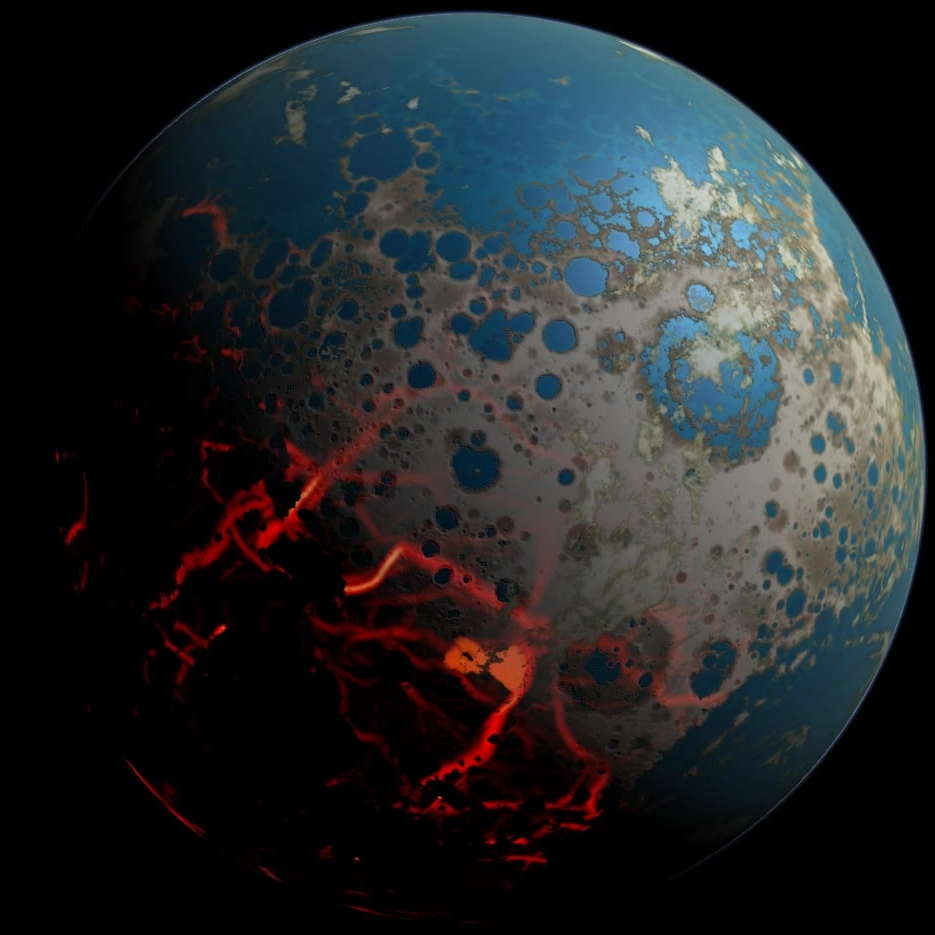
\includegraphics[width=0.5\textwidth]{early-earth.jpg}

\BS
\BS
\Large How do we get from there to here?
\EC

}
{
\setbeamercolor{background canvas}{bg=black}

\frame{
\BC
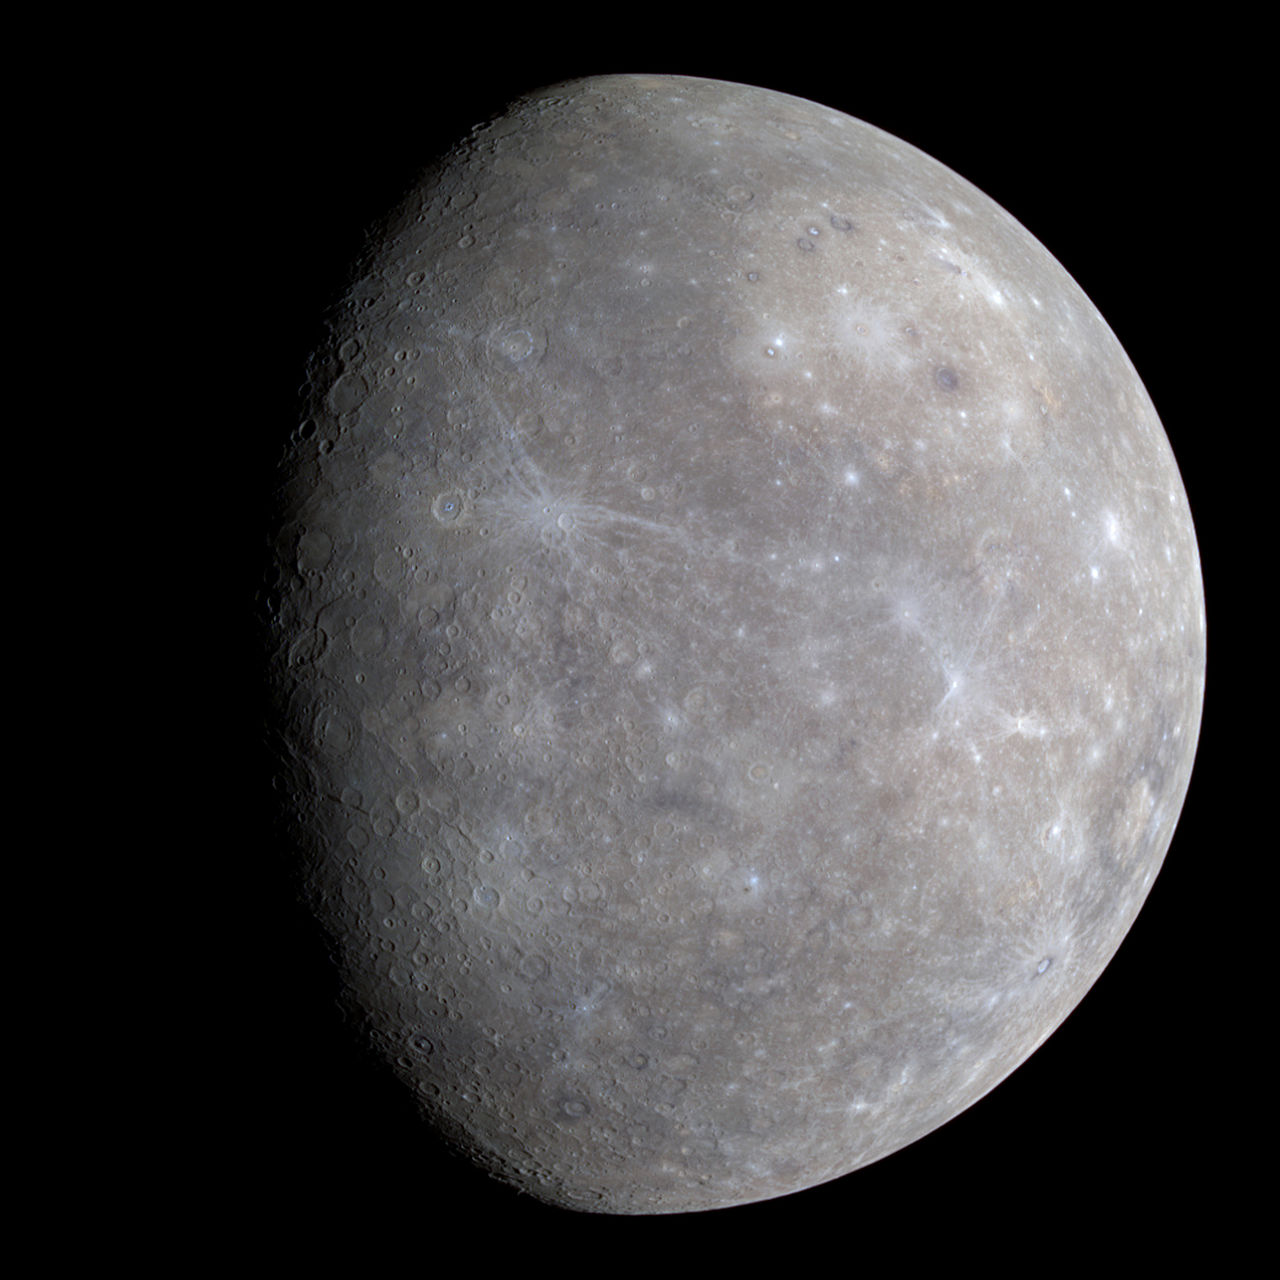
\includegraphics[height=0.49\textheight]{mercury.jpg}
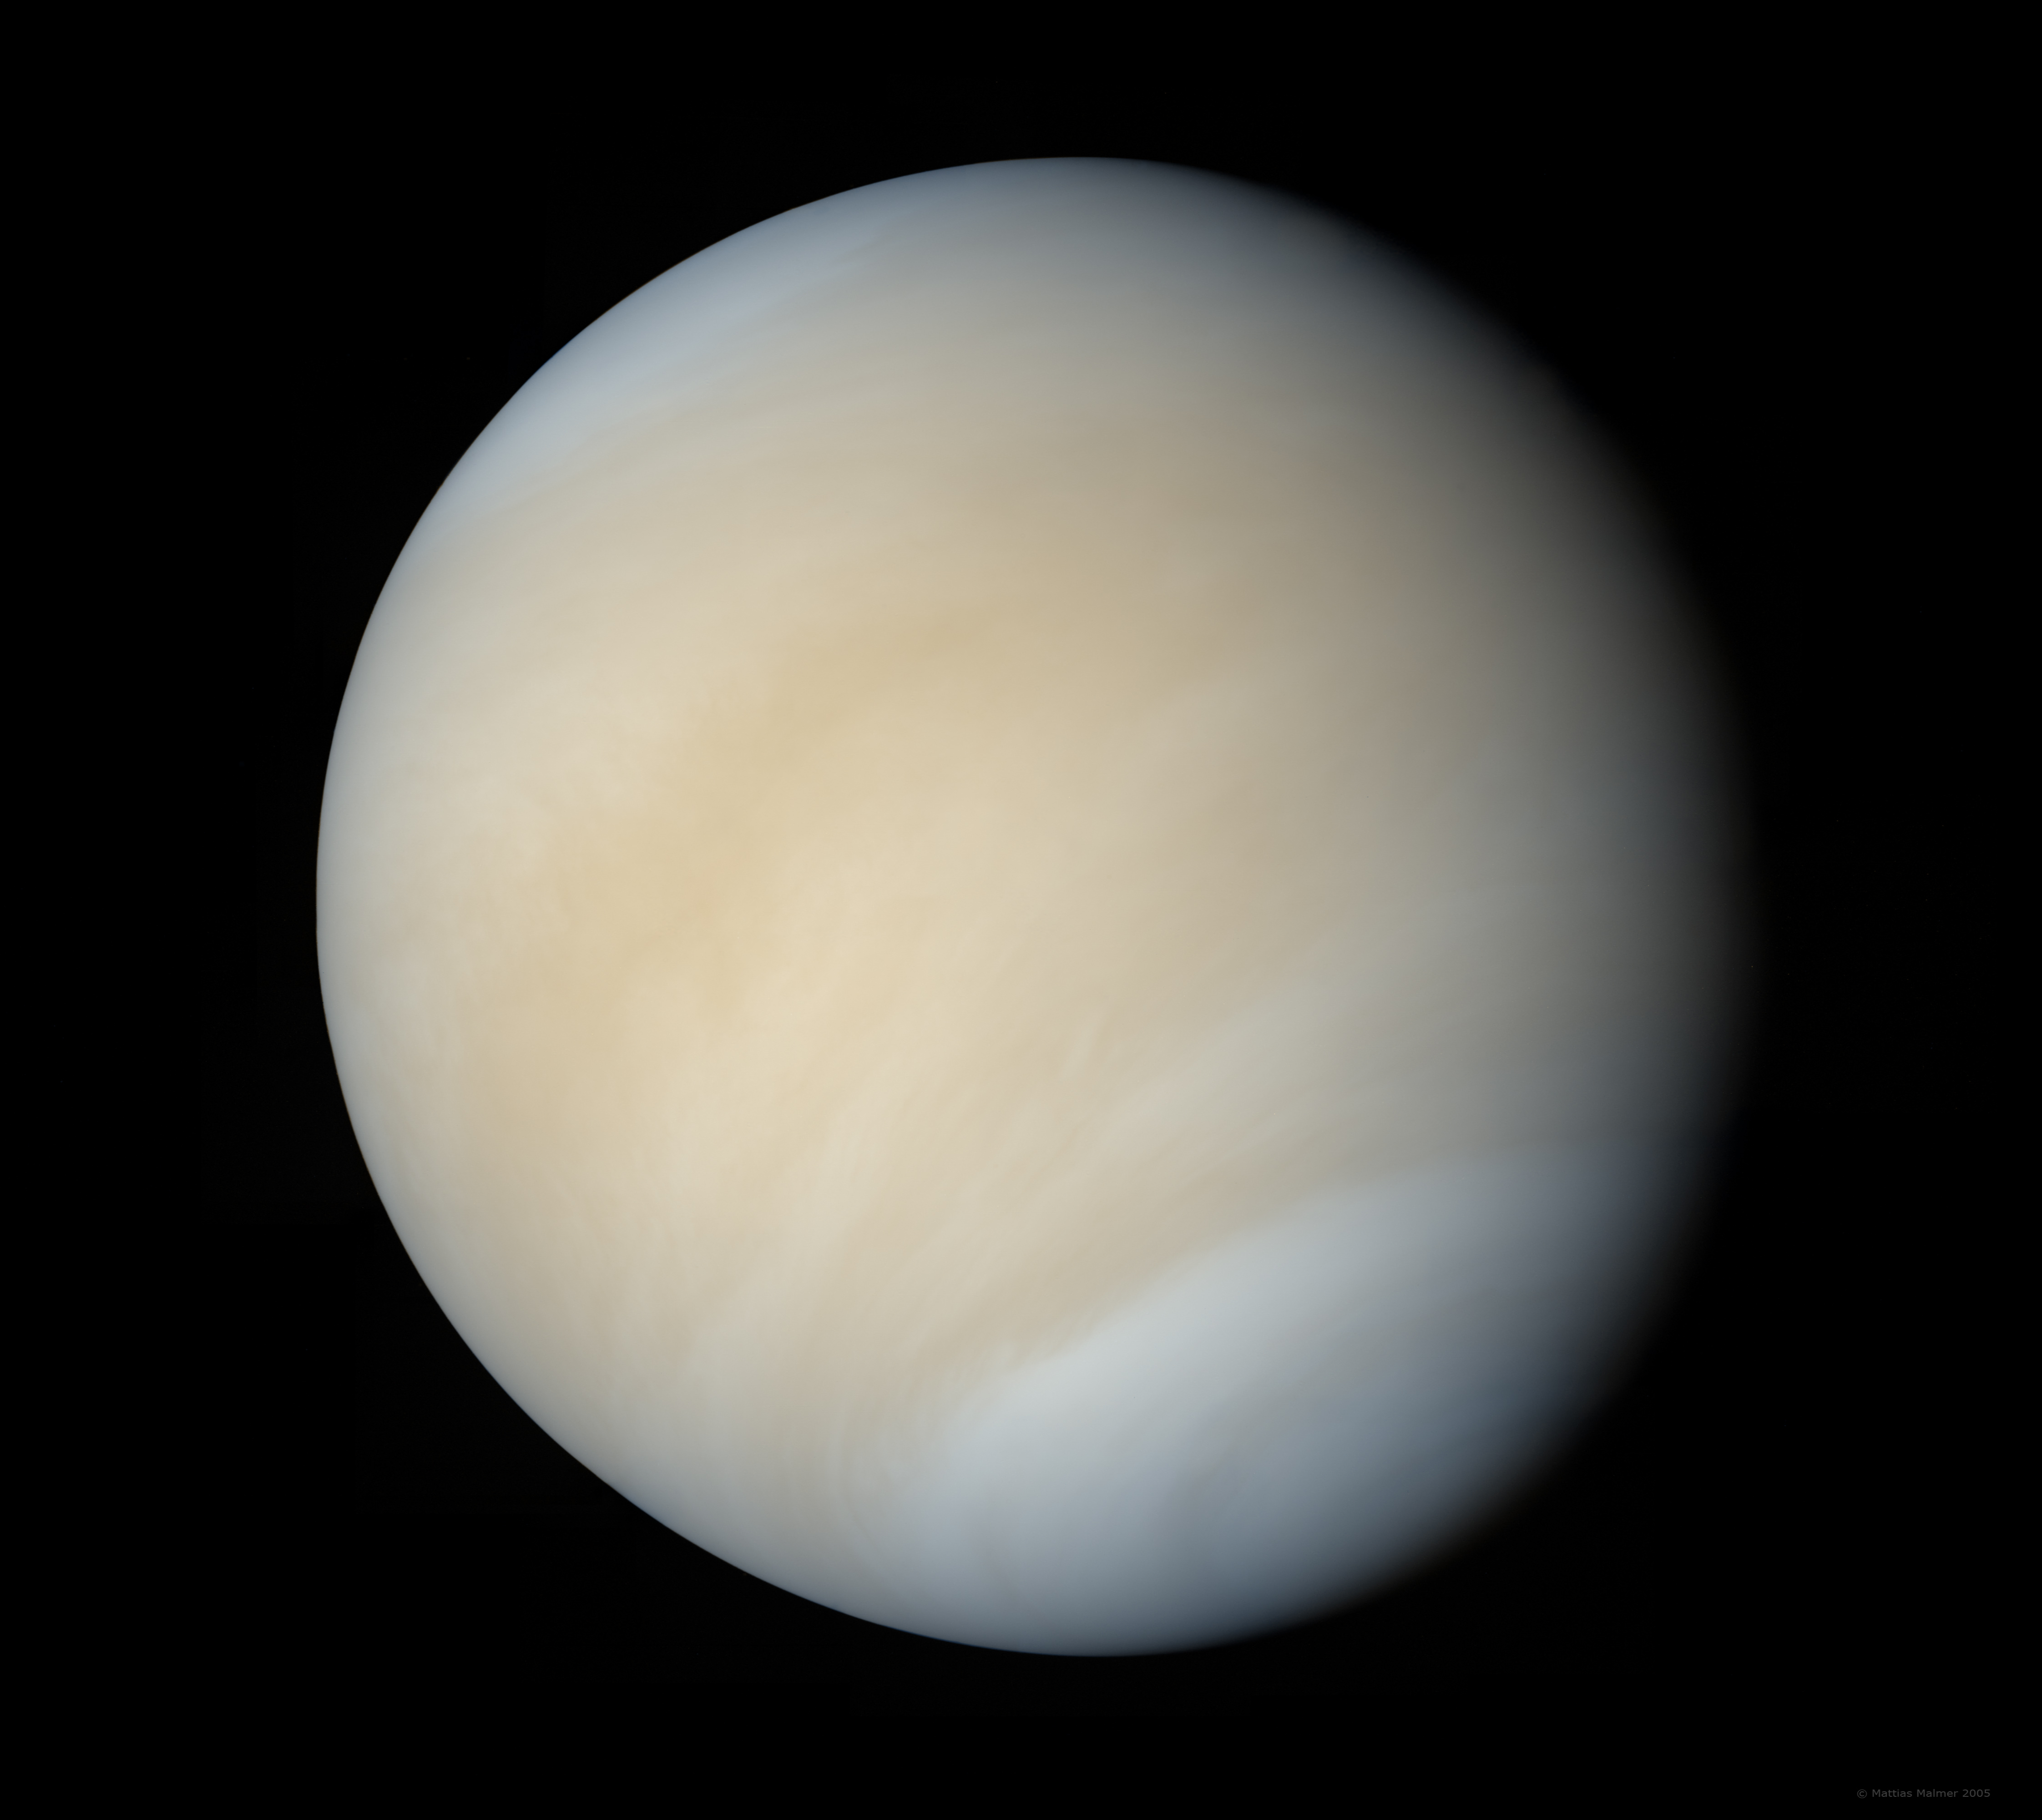
\includegraphics[height=0.49\textheight]{venus.jpg} \\
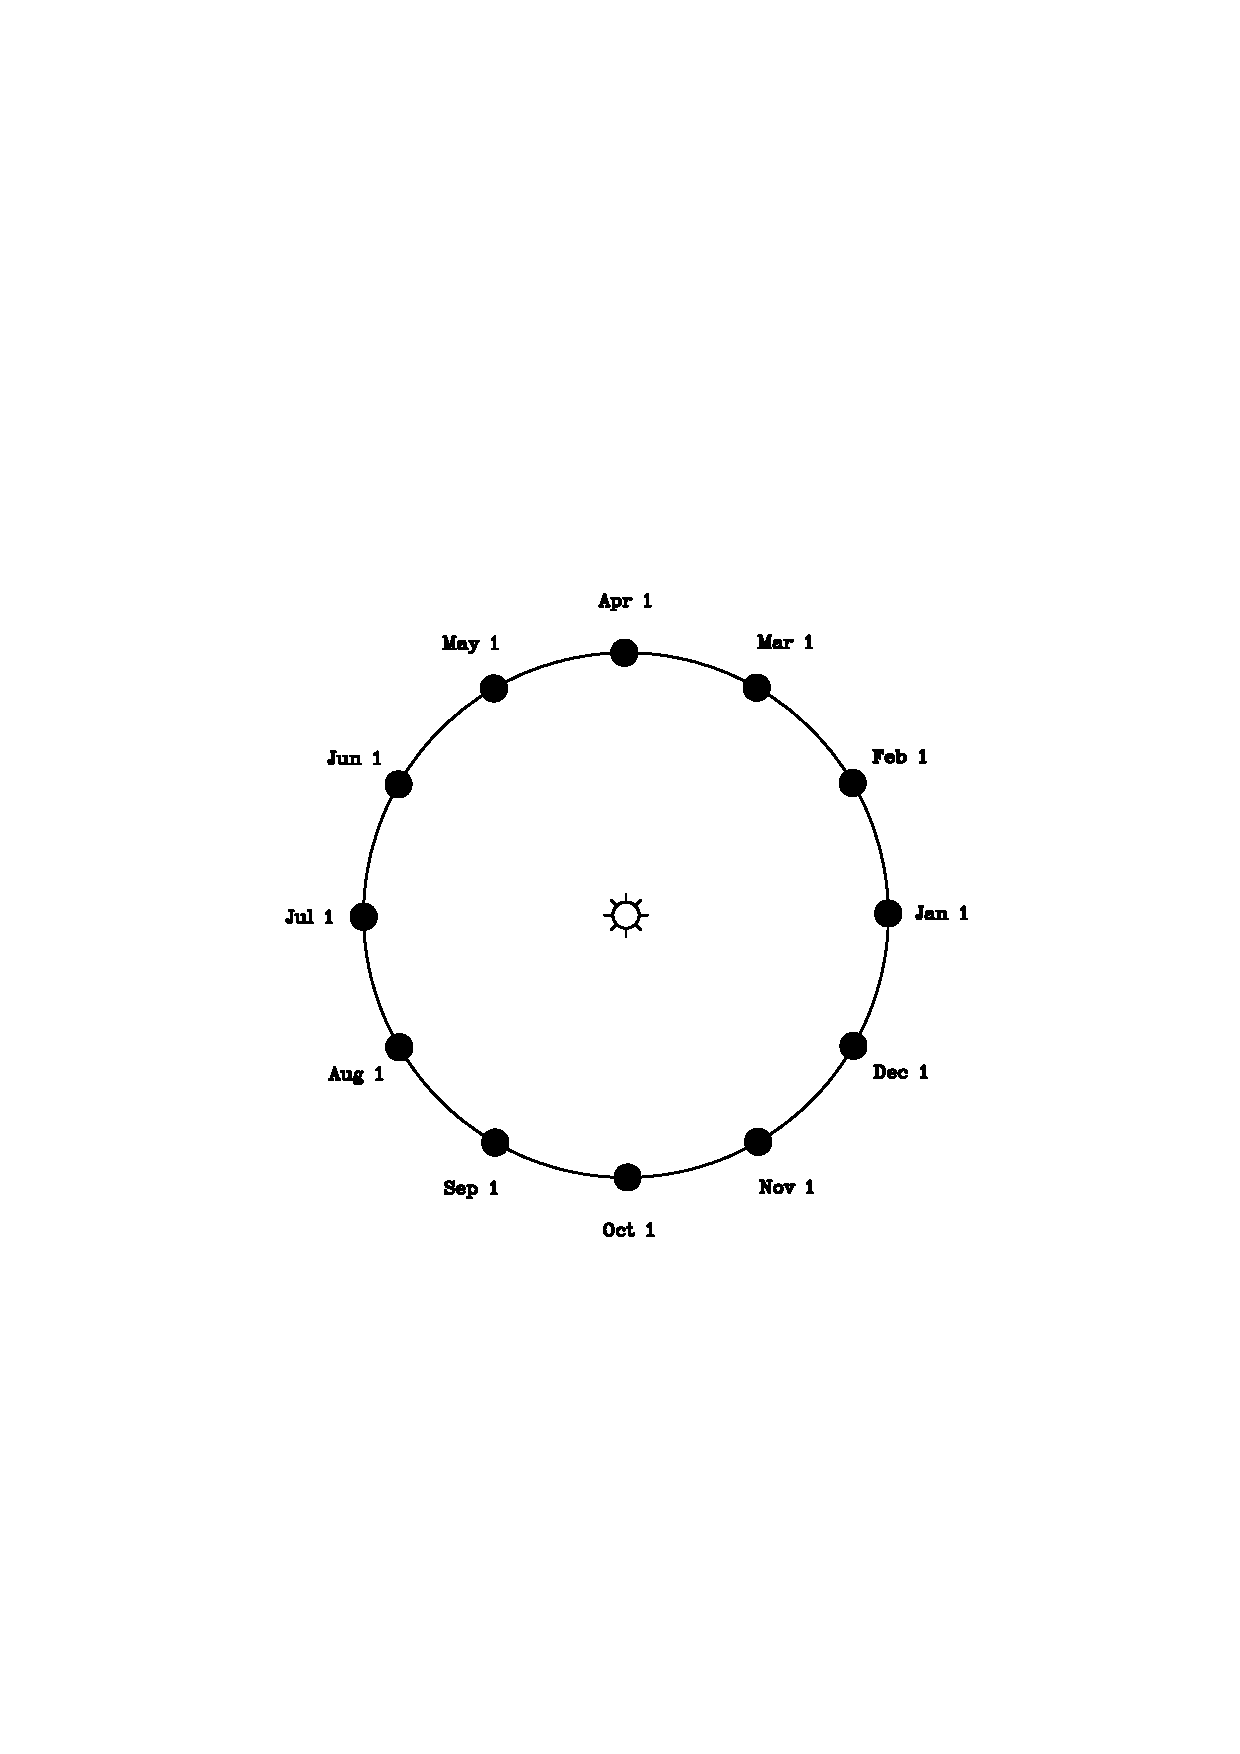
\includegraphics[height=0.49\textheight]{earth.jpg}
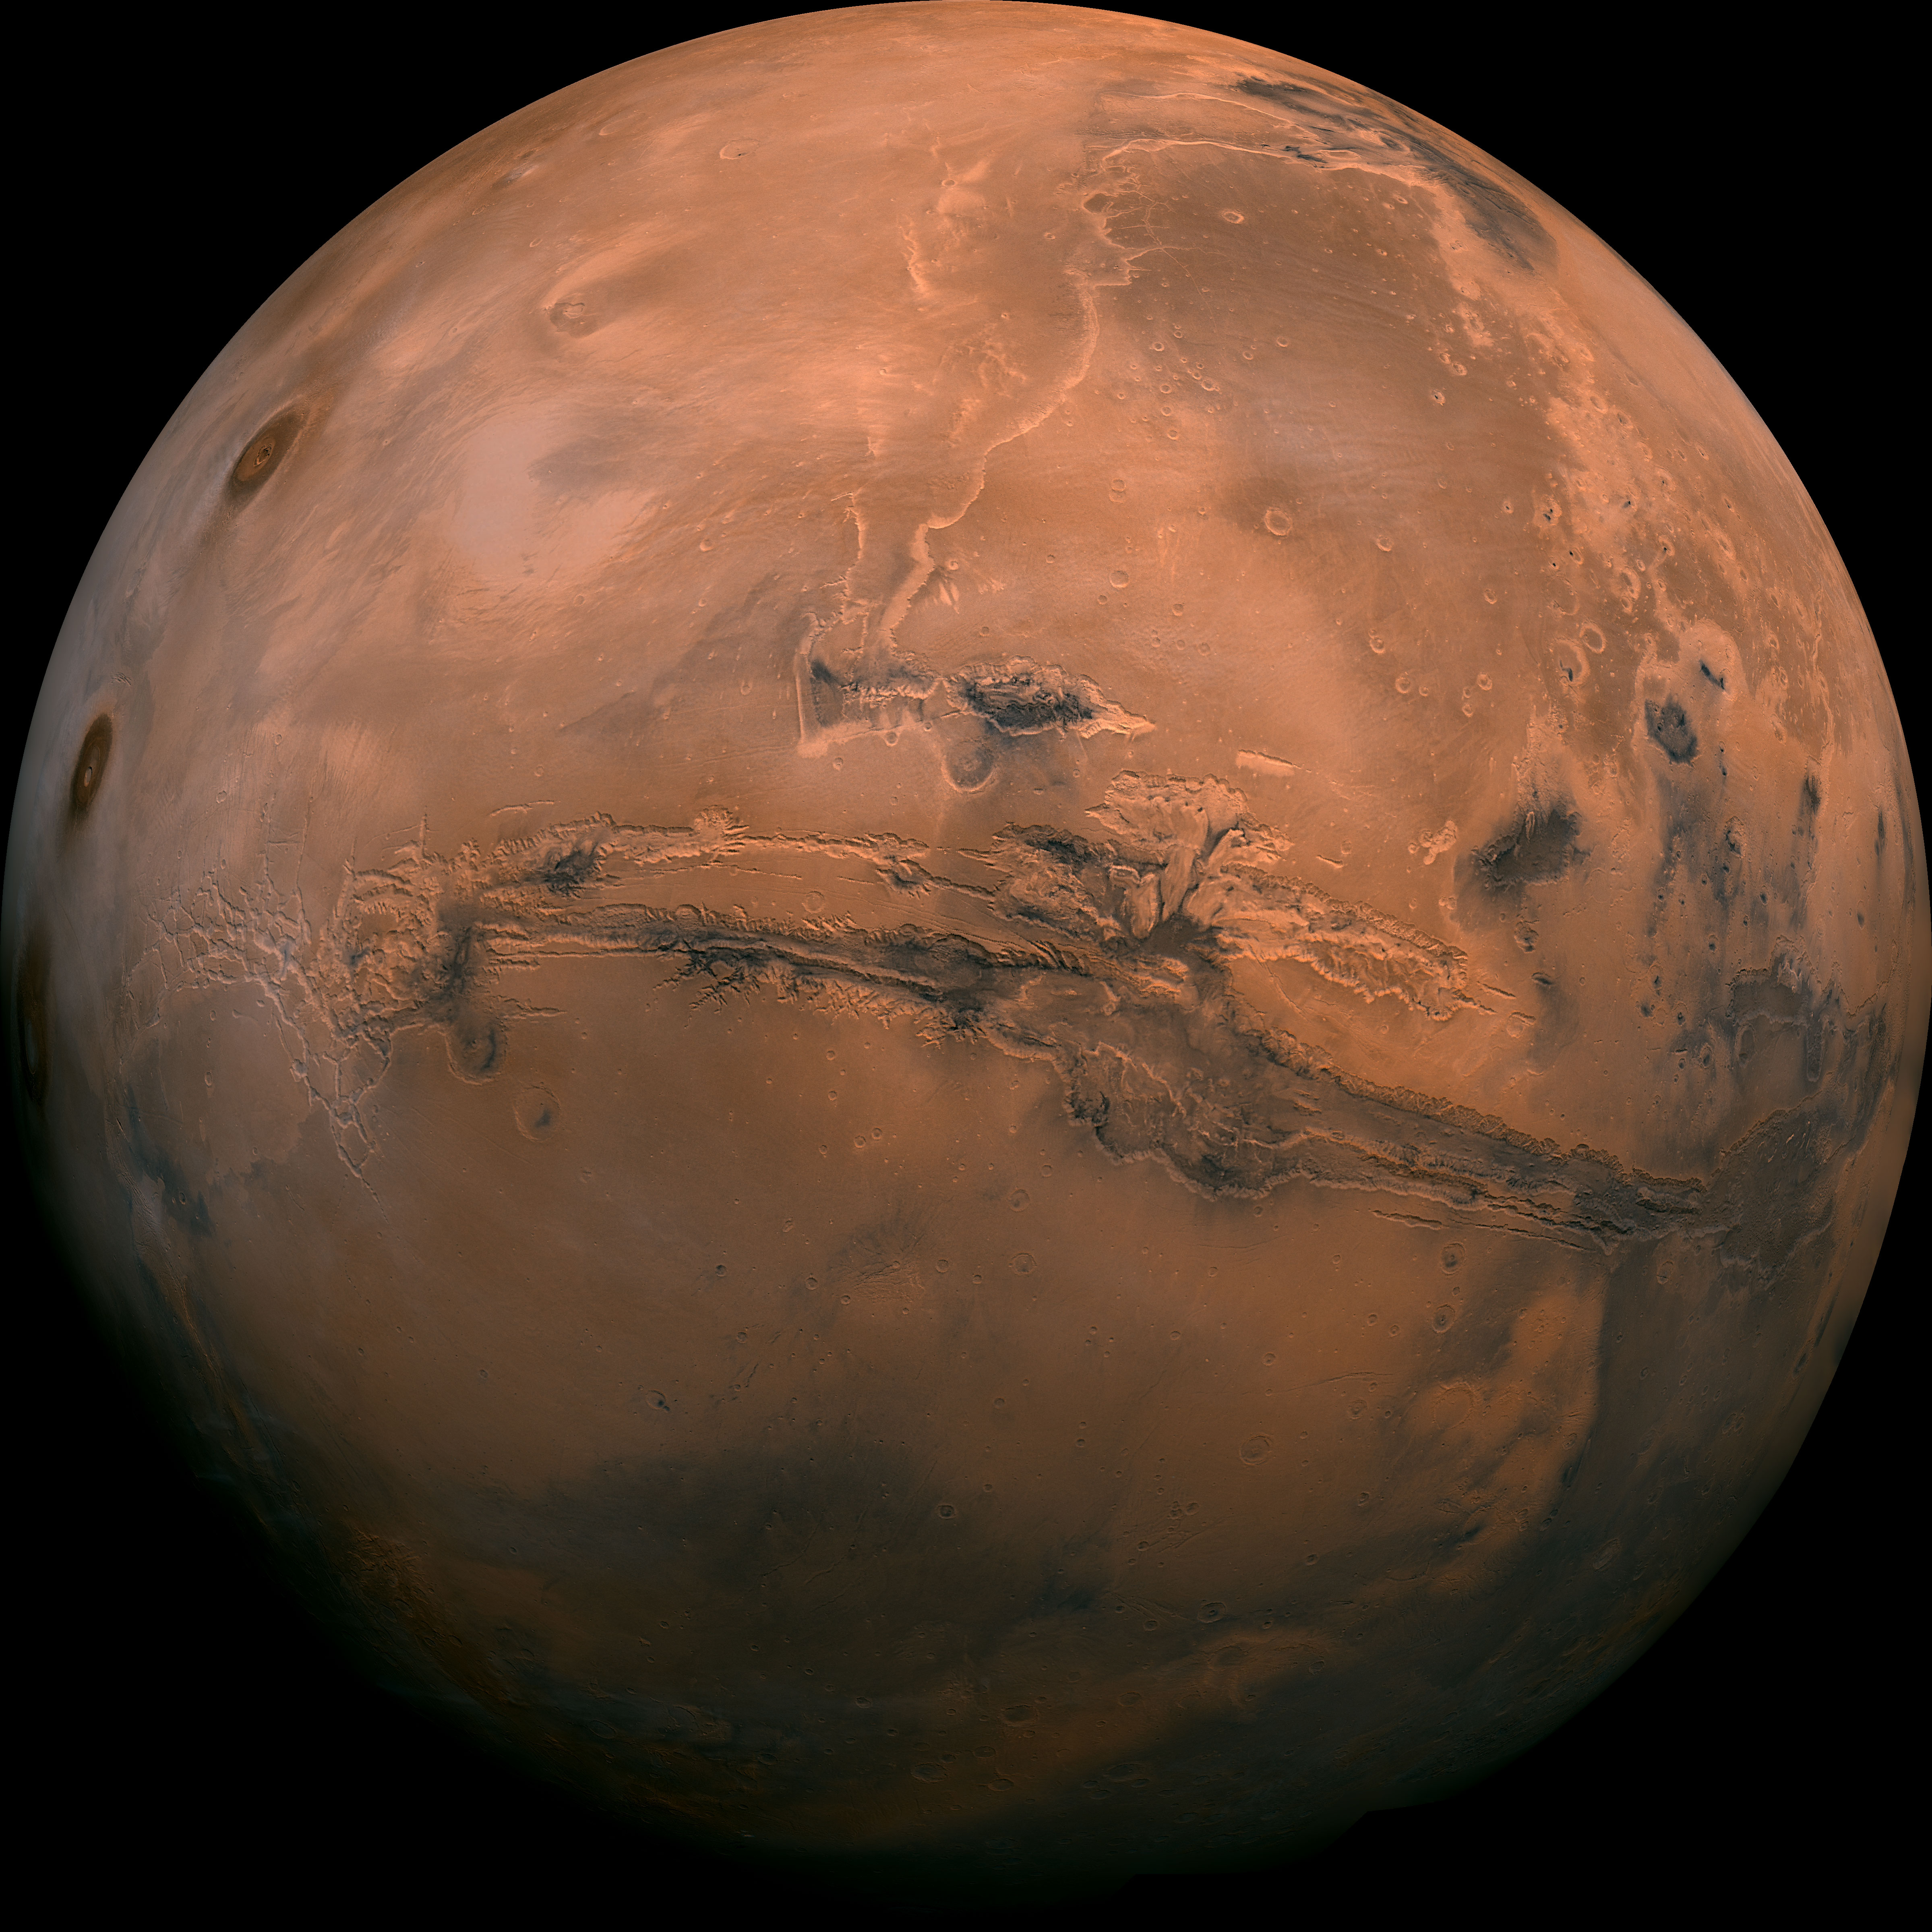
\includegraphics[height=0.49\textheight]{mars.jpg}
\EC

}
}

\frame{\frametitle{\bf A few things to keep in mind}

\Large
\BI
\item Asteroids: any unprotected object gets hit repeatedly (more in early solar system)
\item Our atmosphere is thick enough to burn up many, but not all, asteroids
\item Volcanism:
\BI
\large
\item Hot rocks melt
\item Molten things flow
\item If the core of a planet is hot, it has volcanic activity
\item Radioactive decays of uranium sustain internal heat of planets over billions of years
\EI
\EI
}

\frame{

% Please add the following required packages to your document preamble:
% \usepackage{booktabs}
\BC
\begin{tabular}{@{}l | lllll@{}}
\toprule
        & Orbit (AU) & Radius (km) & Temp (actual) & Temp (pred.) & Volcanism? \\ \midrule
Mercury & 0.39                & 2440        & 700 / 100 K   & 439 K & Long ago                \\
Venus   & 0.72                & 6051        & 740 K         & 321 K & Yes                \\
Earth   & 1                   & 6378        & 290 K         & 273 K & Yes                \\
Mars    & 1.52                & 3397        & 220 K         & 222 K & In the past              \\ \bottomrule
\end{tabular}

\BS
\BS

\begin{tabular}{@{}l | lllll@{}}
\toprule
        & Orbit (AU) & $\Delta$ Temp & Atmosphere                  & Atmospheric pressure \\ \midrule
Mercury & 0.39                       & small               & None                        & None                 \\
Venus   & 0.72                       & +419 K            & $\rm CO_2$                  & 92 atm               \\
Earth   & 1                          & +17 K            & $\rm N_2; O_2; CO_2; H_2 O$ & 1 atm                \\
Mars    & 1.52                       & -2 K            & $\rm CO_2; N_2; Ar$         & 0.006 atm            \\ \bottomrule
\end{tabular}
\EC
}

\frame{
\BC
\large
Mercury, the fleet messenger god, whizzing around the Sun...

\BS

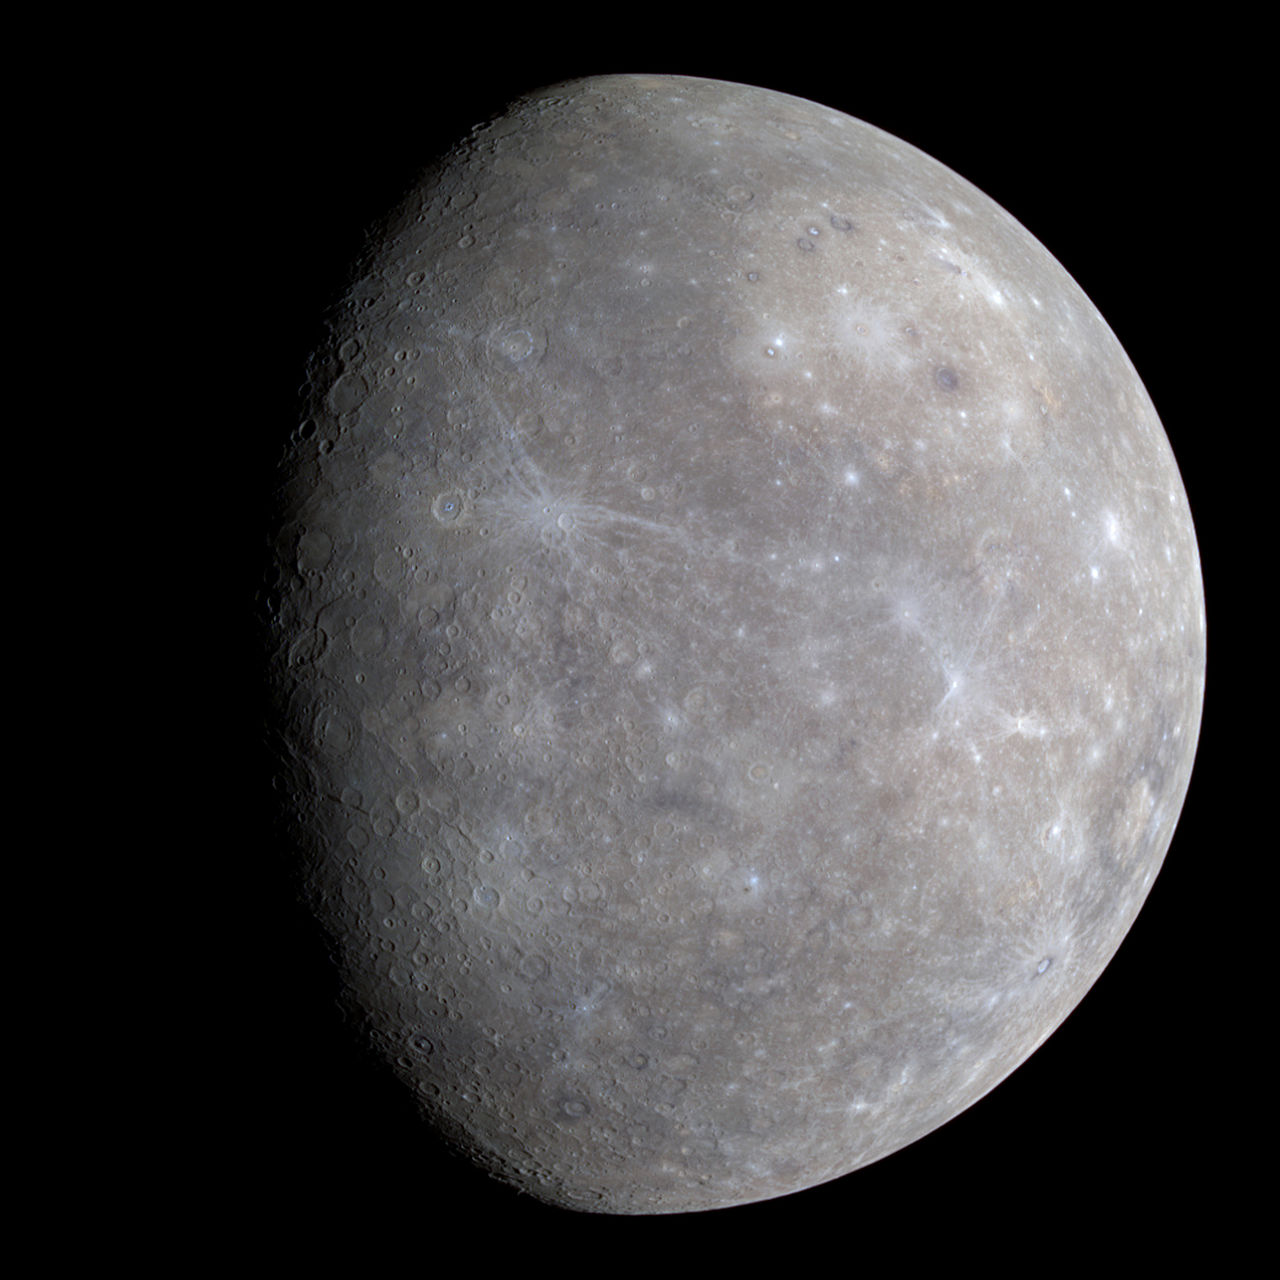
\includegraphics[width=0.5\textwidth]{mercury.jpg}\hspace{0.05\textwidth}
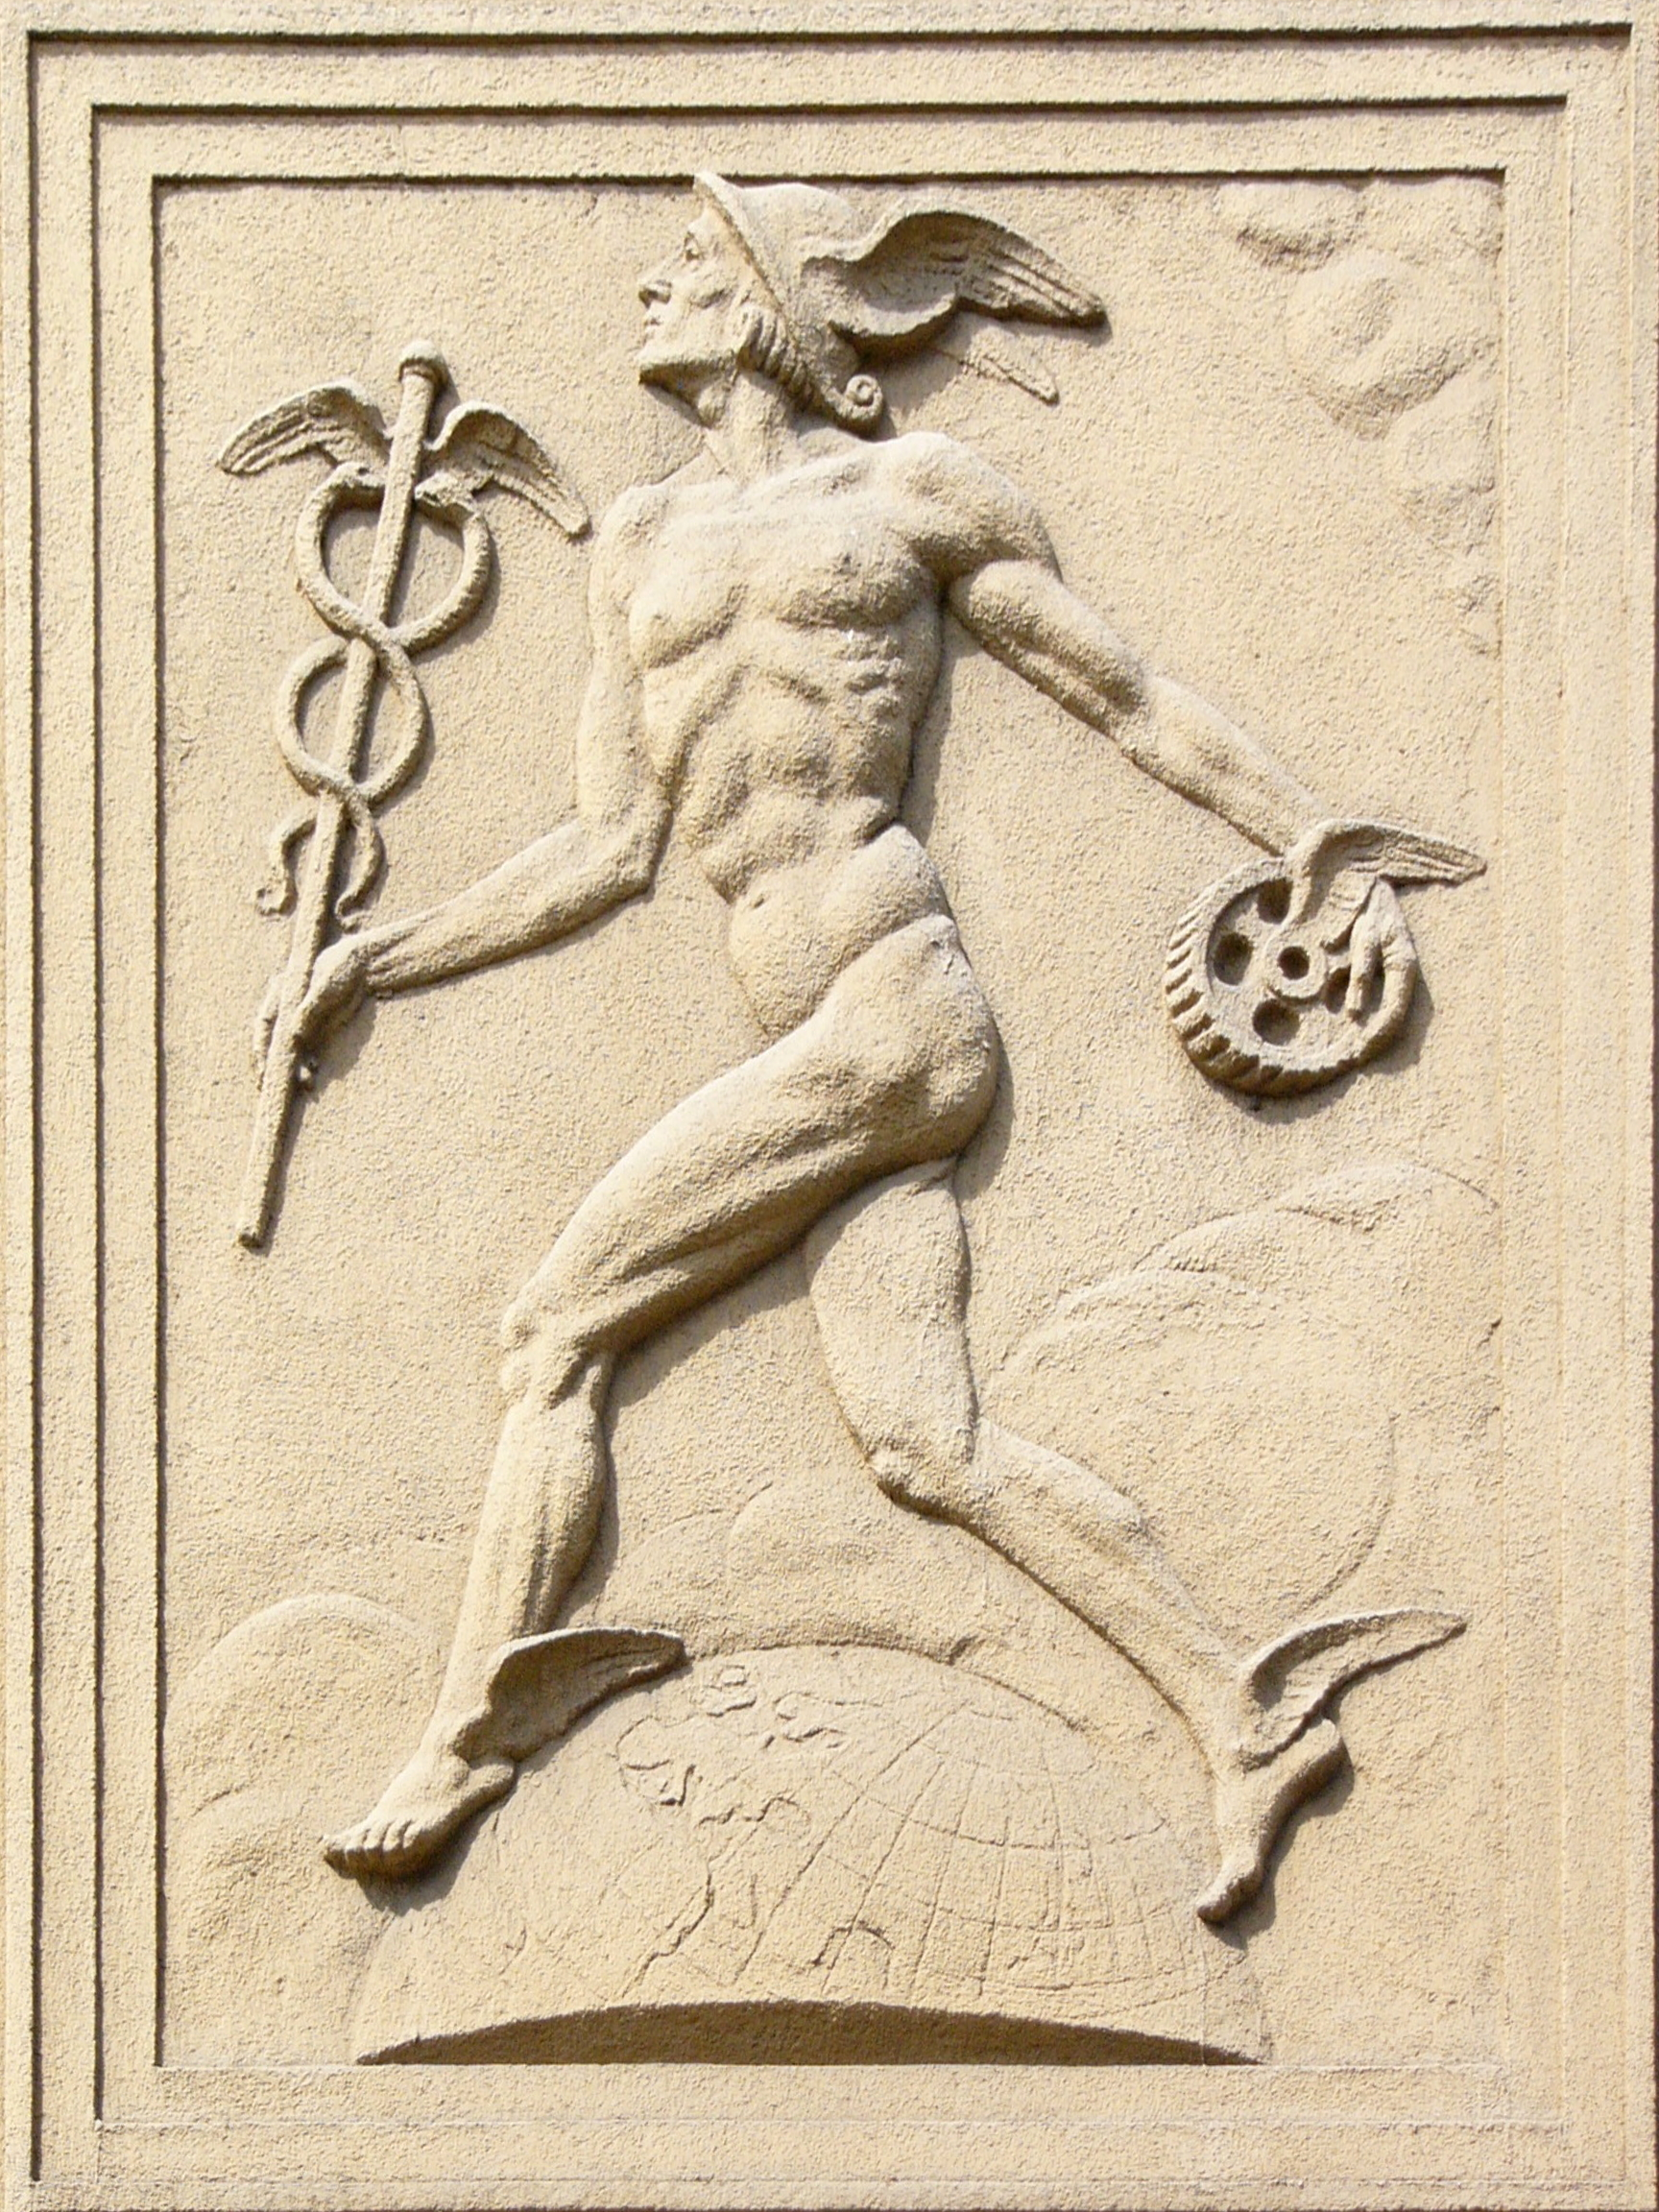
\includegraphics[width=0.4\textwidth]{mercury-relief.jpg} \\


\BS

\url{https://www.youtube.com/watch?v=CilfBWvCSXI}
\EC
}

\frame{\frametitle{\bf Agile, lively Mercury...}

\large

Mercury's surface is pockmarked with craters. This tells us:

\BI 
\item It clearly has been hit by asteroids.
\item It didn't have an atmosphere when this happened
\item No weathering, geologic activity, or the like has taken place since
\pause
\item Mercury is a dead rock. It's interesting if you like rocks...
\EI
\pause
\BC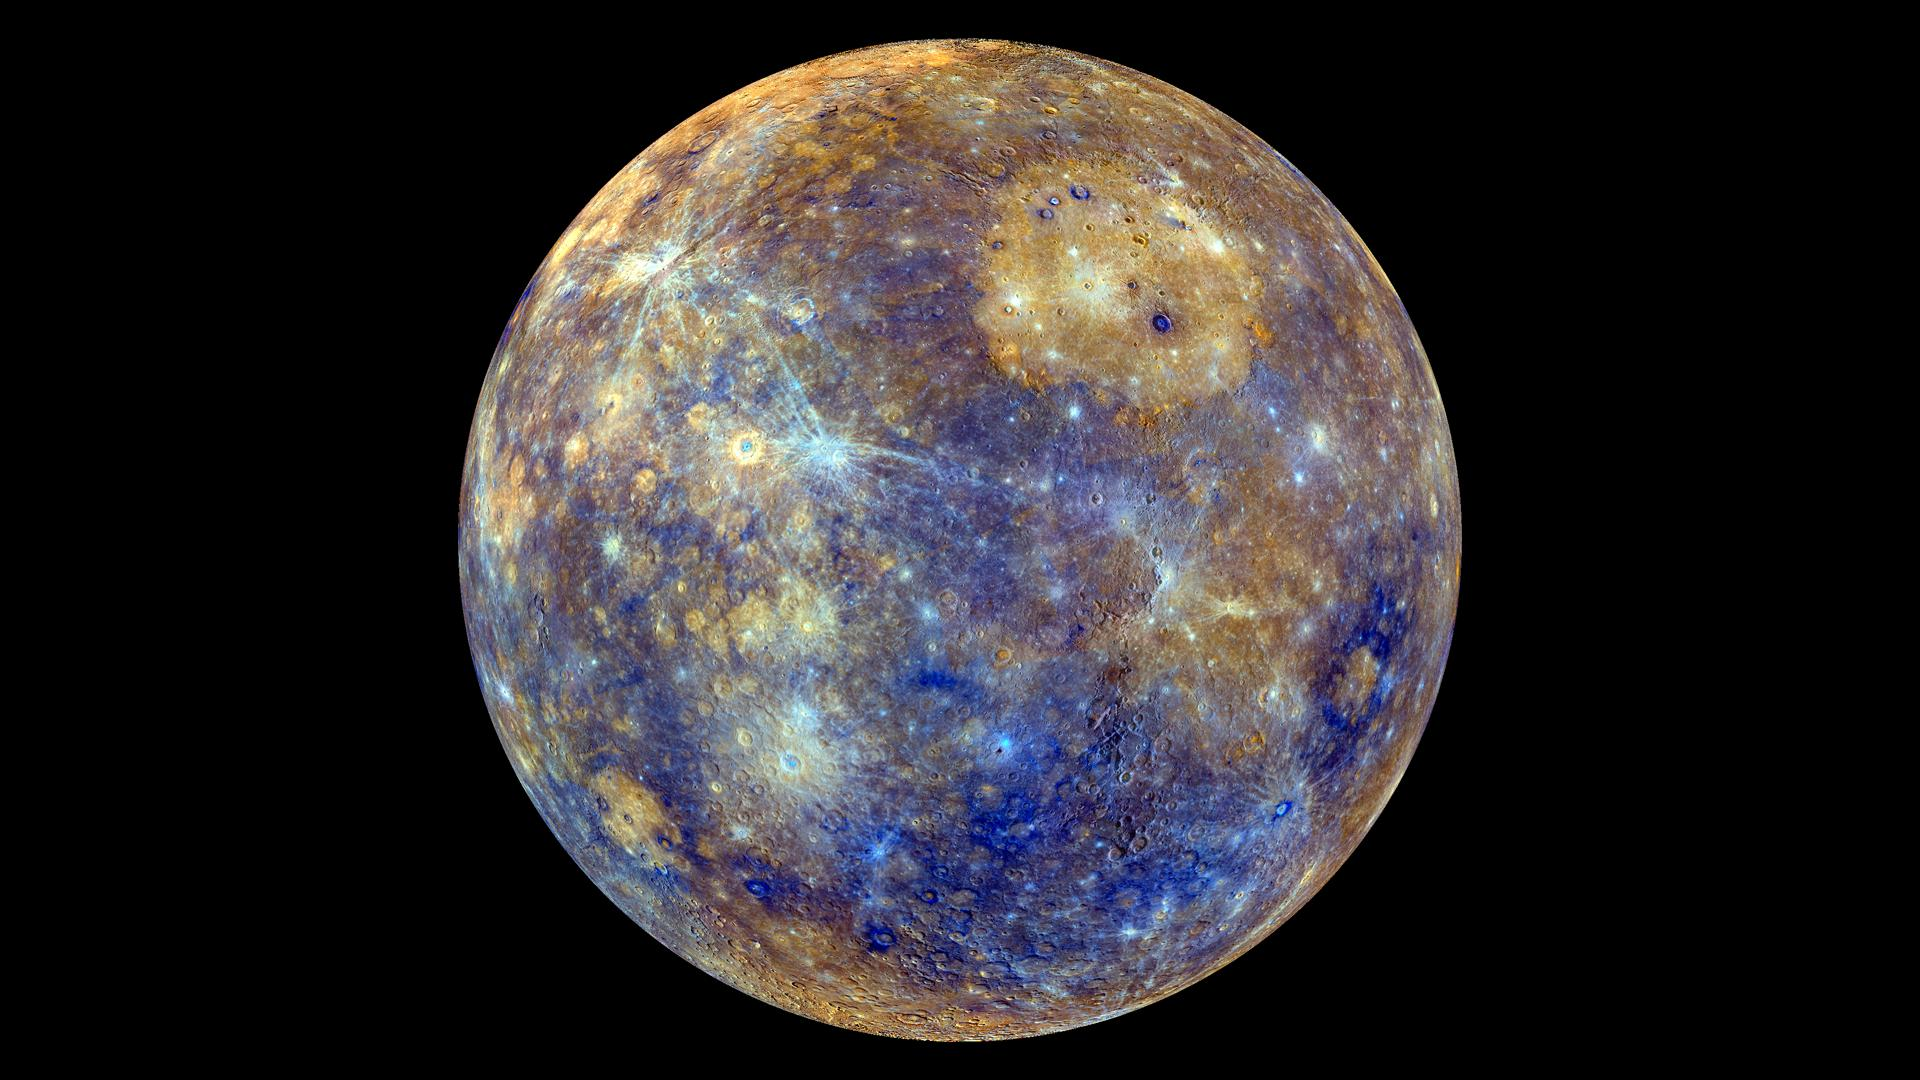
\includegraphics[width=0.6\textwidth]{mercury-color.jpg}\EC
}

\frame{

\BC
\large
Mars, the cruel god of war... 

\BS

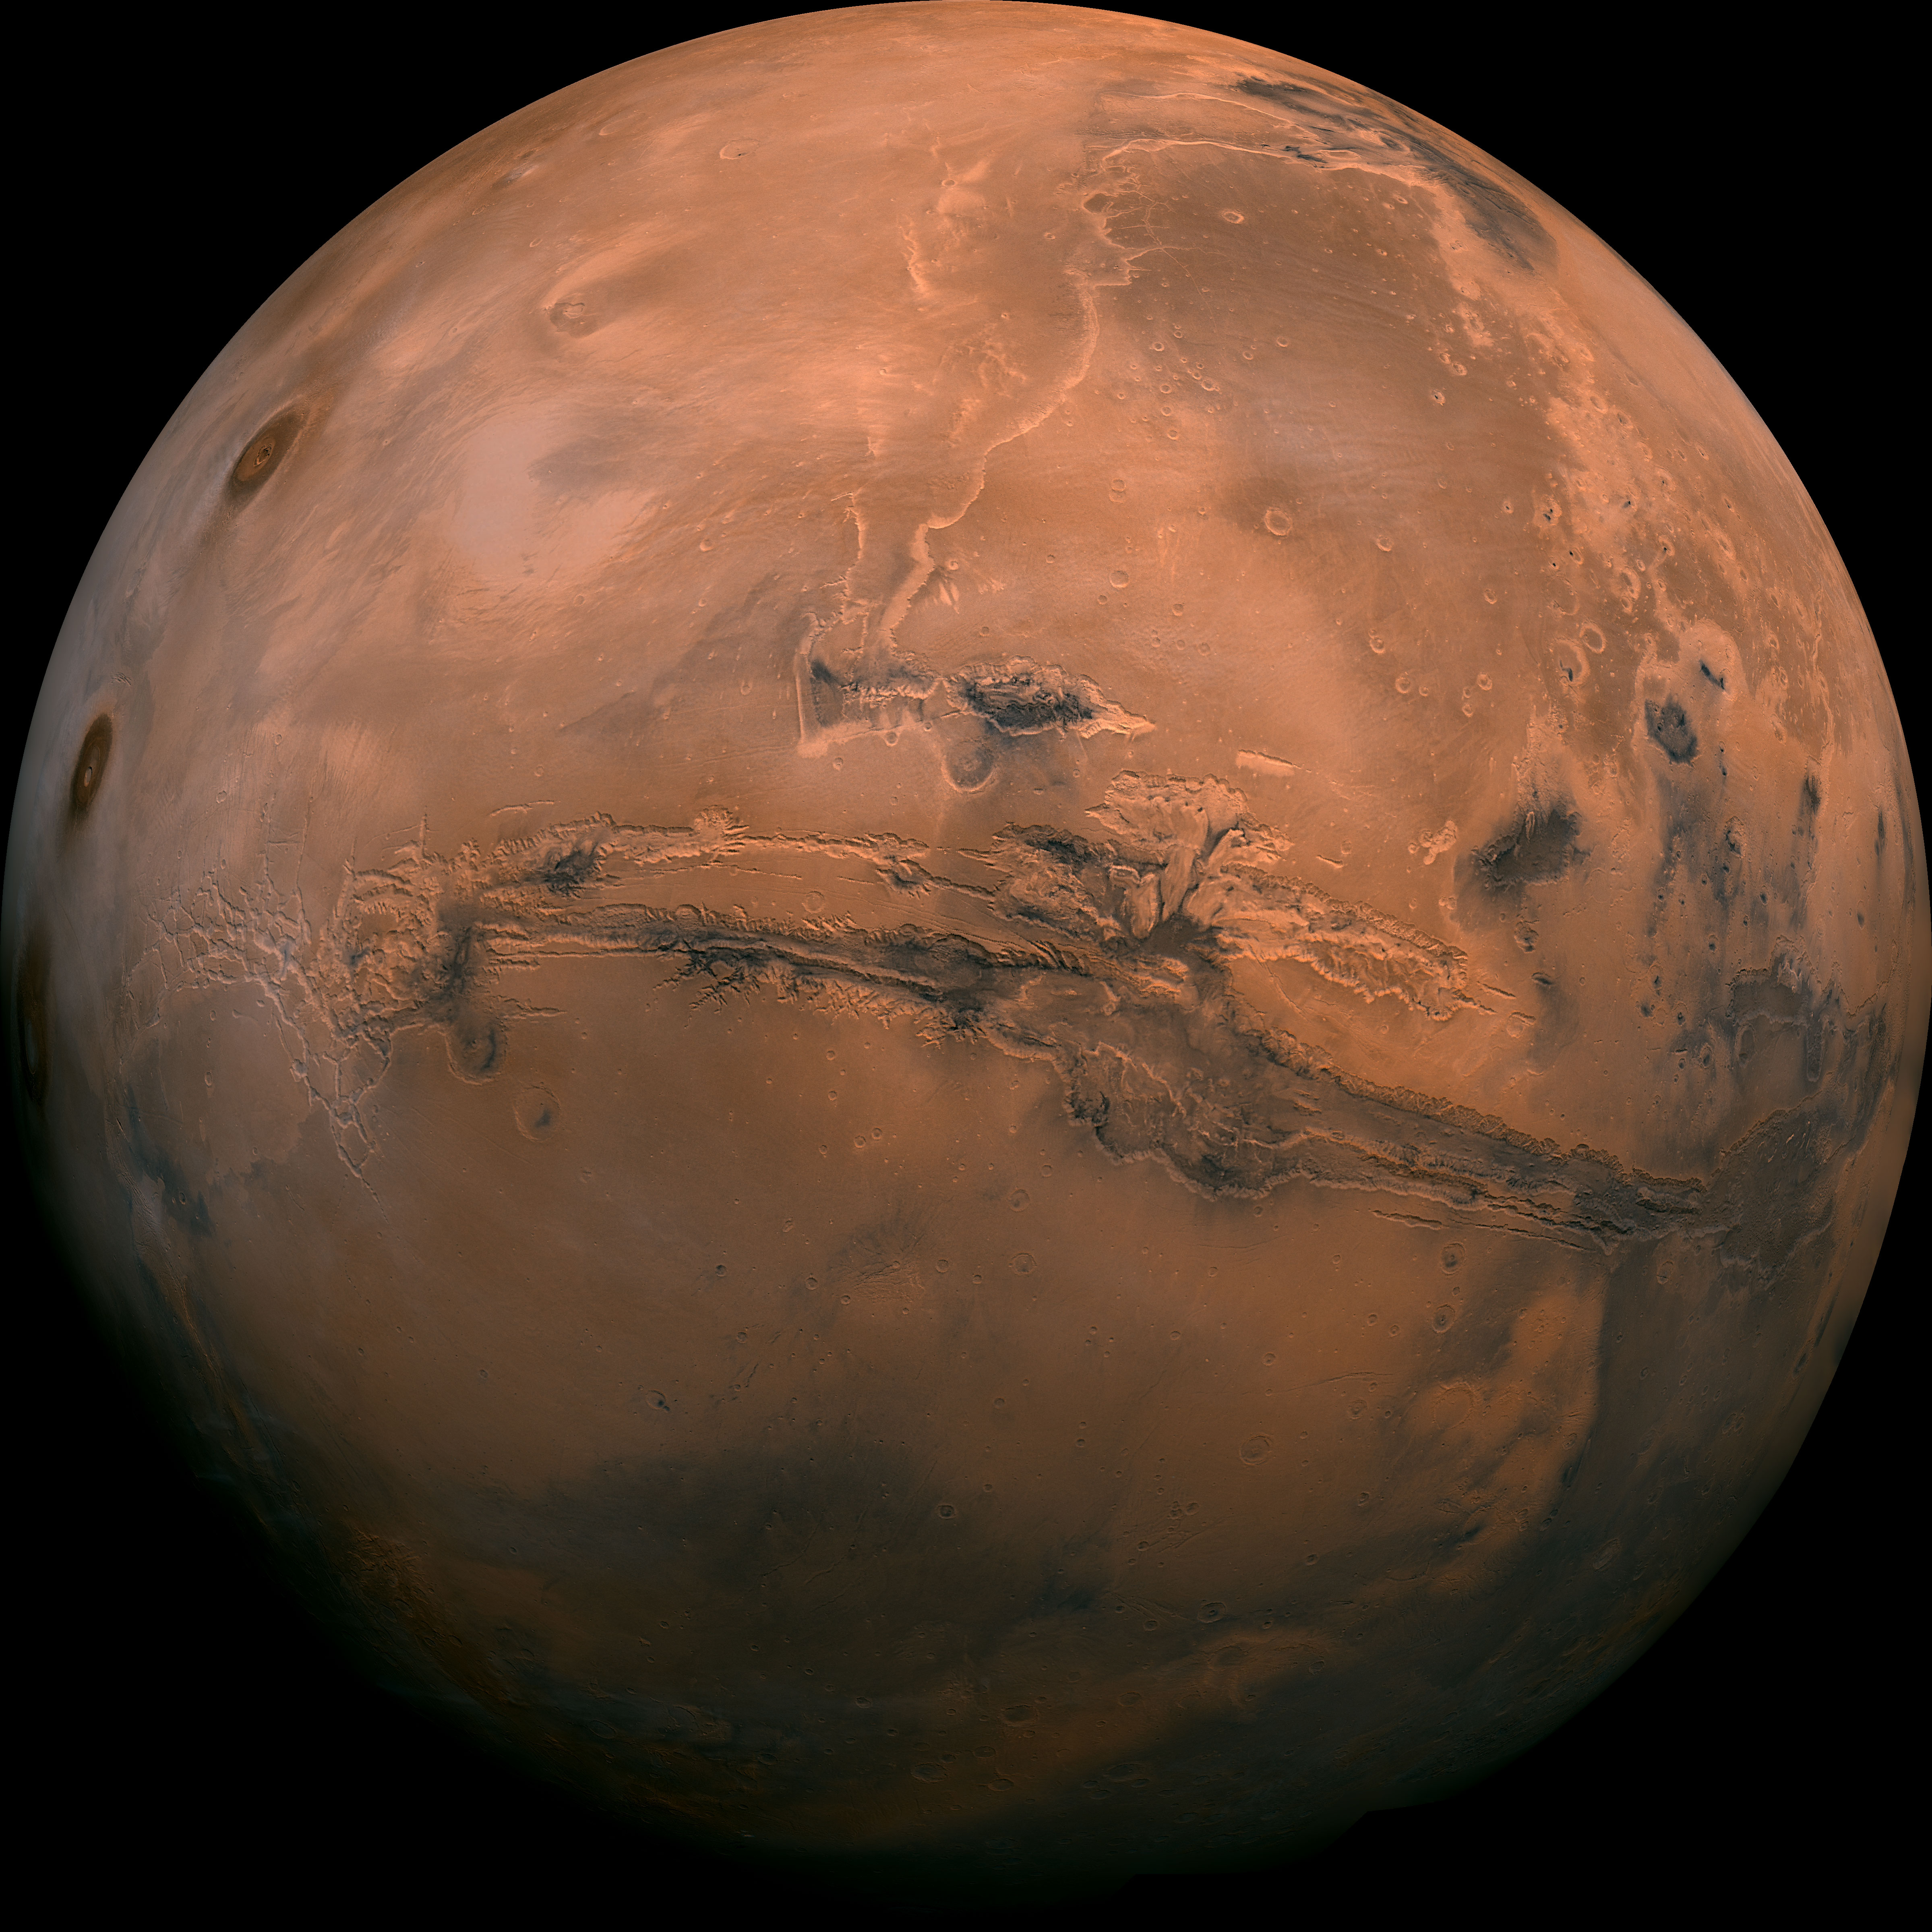
\includegraphics[width=0.55\textwidth]{mars.jpg}\hspace{0.1\textwidth}
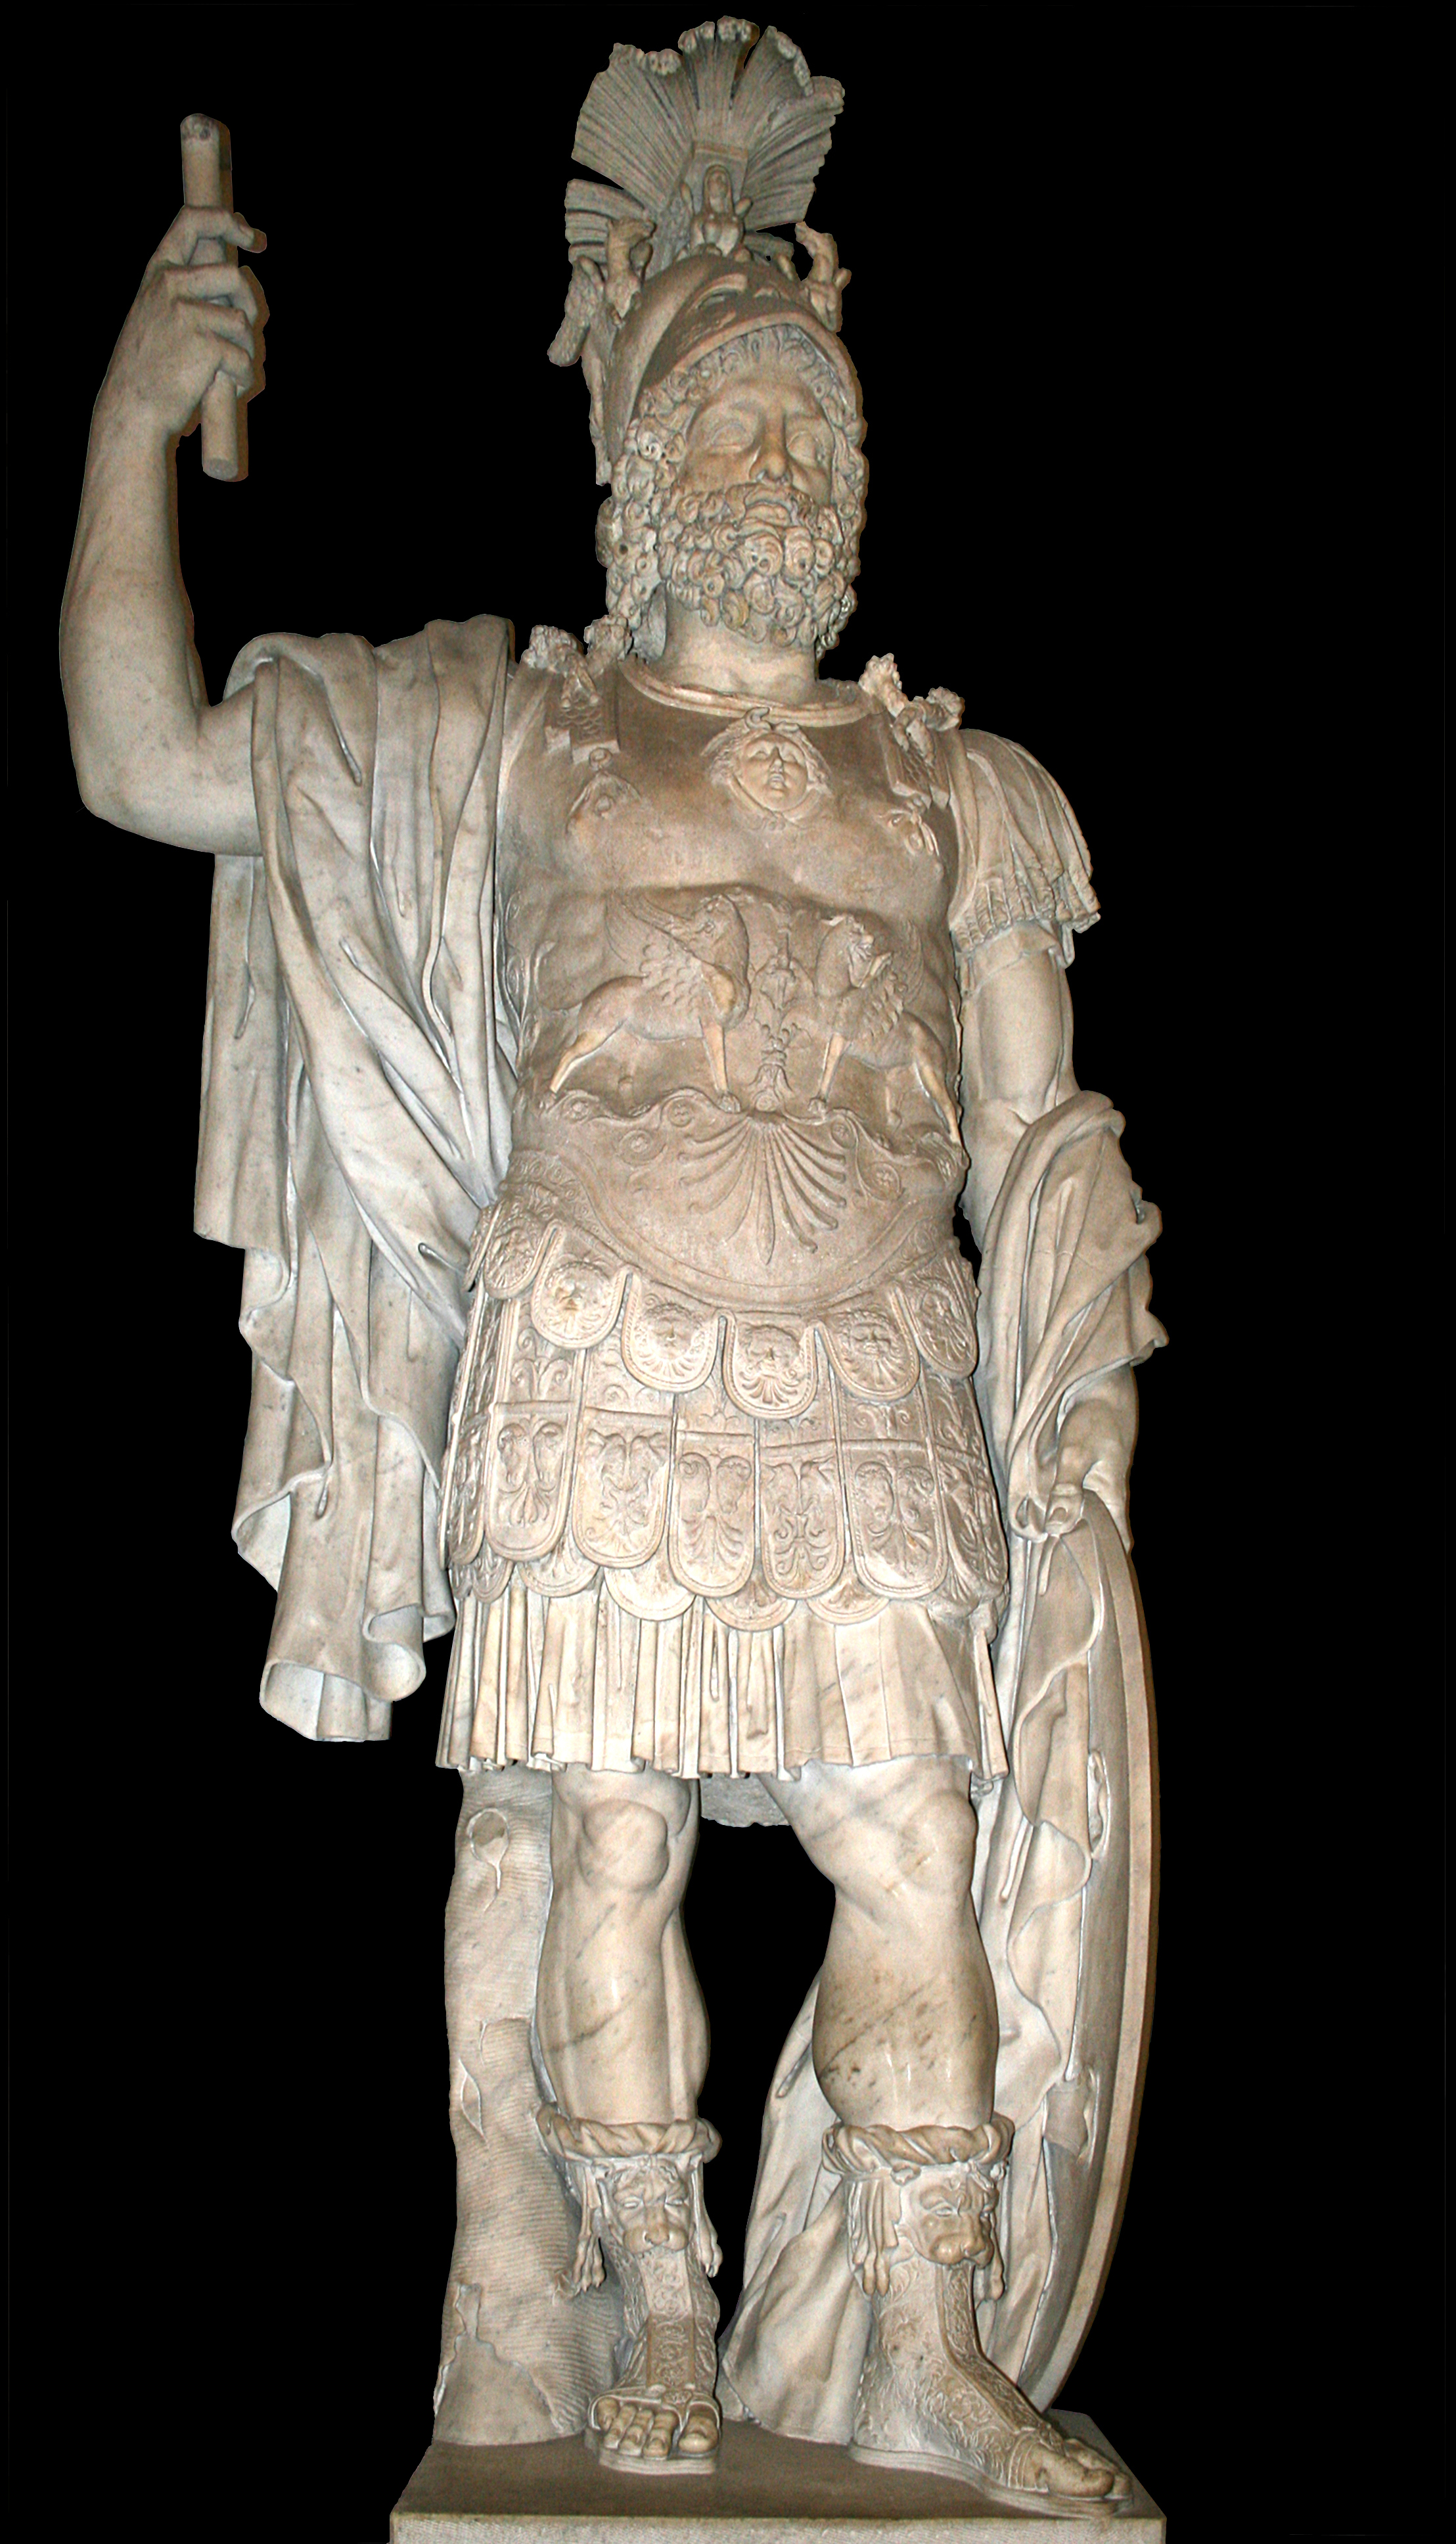
\includegraphics[width=0.30\textwidth]{mars-statue.jpg} \\

\url{https://www.youtube.com/watch?v=cXOanvv4plU}
\EC
}

\frame{\frametitle{\bf Bloodthirsty, violent Mars...}

We've sent robots to Mars that have explored it some detail. We find:

\BI
\item Rocks with rust in them, making it {\color{Red}red}
\item Only a thin atmosphere, mostly $\rm CO_2$
\item Large volcanoes, none active
\item Evidence of interior heat, but not like Earth and Venus
\item Evidence that liquid water once ran on its surface
\item Evidence that it once had an atmosphere of water and $\rm CO_2$
\item Evidence that was once much warmer than it is today
\pause
\item ... what happened?
\EI
}

\frame{\frametitle{\bf Rusty, peaceful Mars...}

\BI 
\item Something happened around three billion years ago
\item Mars lost its atmosphere
\BI
\item Decline in interior heat $\rightarrow$ less volcanism?
\item Solar wind stripping the atmosphere away?
\item Still an area of active research
\EI
\item This caused it to cool (no more greenhouse effect!)
\pause
\item Now Mars' surface mostly contains memories...
\pause
\item ... and robots!
\EI
}

\frame{\frametitle{\bf Mars, the robots' domain...}

\large
\BC NASA sent two small rovers to Mars that landed in 2004. \EC

\BS

\BI
\item These two little robots, named {\it Spirit} and {\it Opportunity}, were supposed to last 90 sols...

\item {\it Spirit:} stuck after 2274 Martian days (6.4 years). \url{https://xkcd.com/695/}
\item {\it Opportunity:} unresponsive after a dust storm after 5,250 Martian days (14.7 years)
\EI

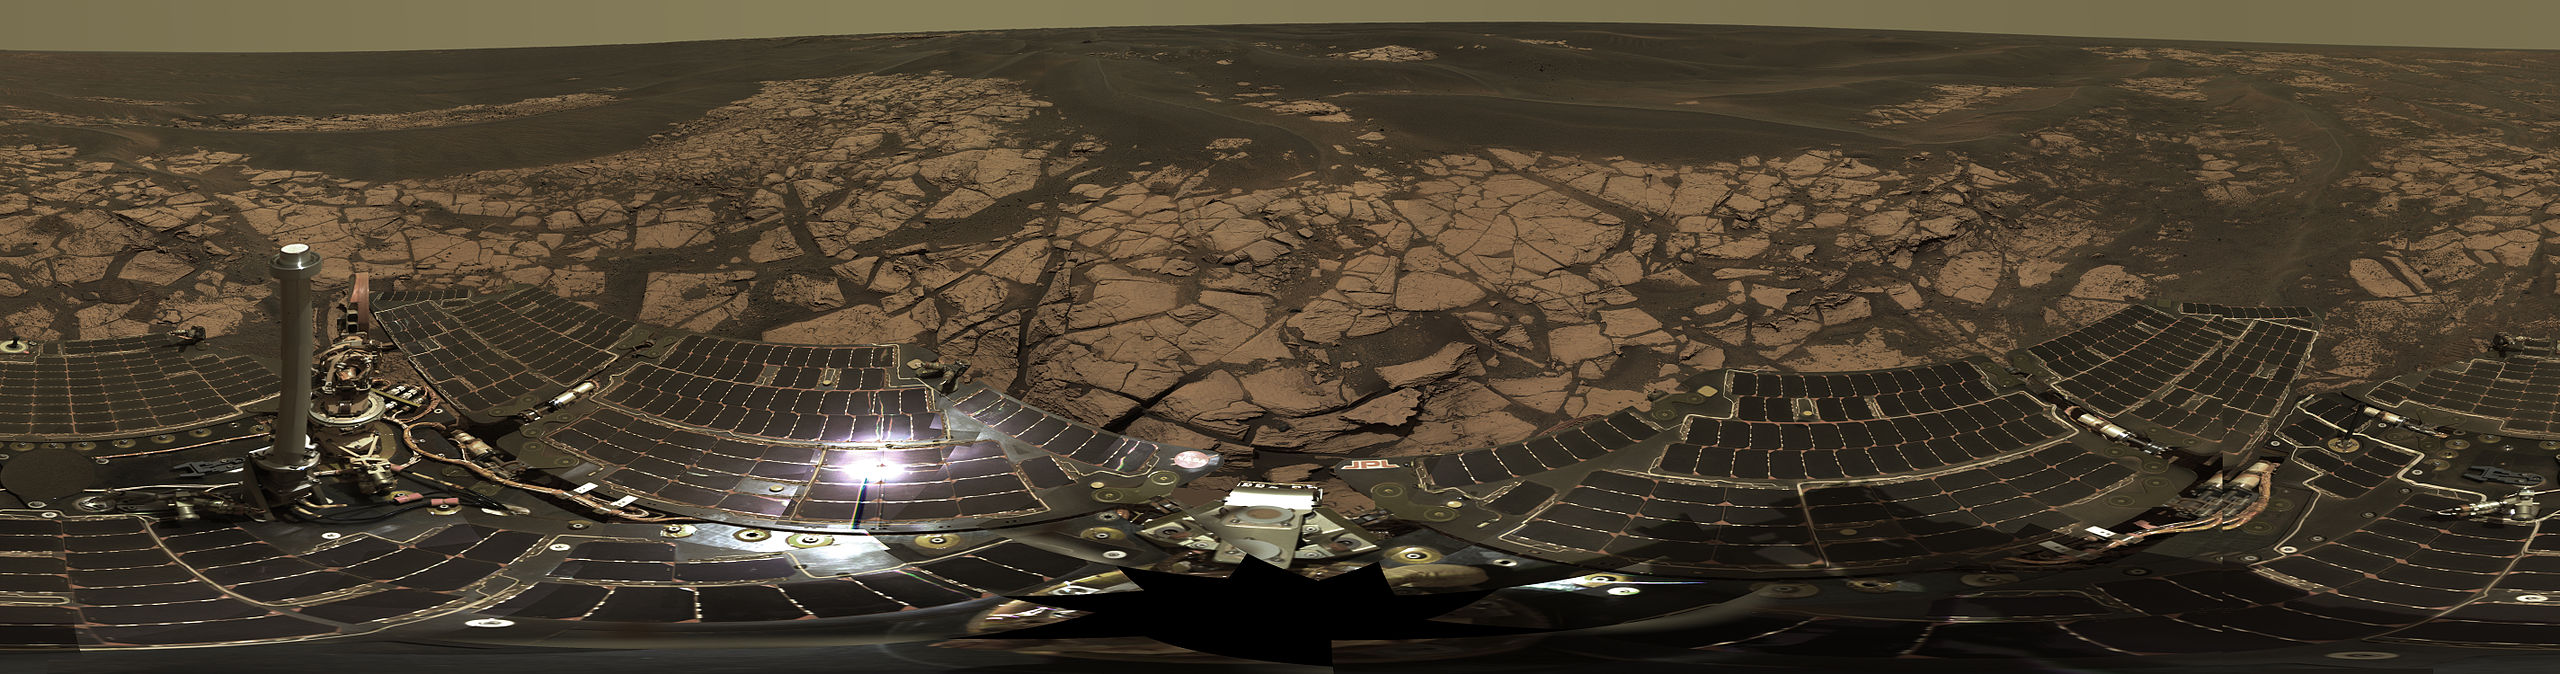
\includegraphics[width=\textwidth]{erebus.jpg}

}





\frame{

\BC
\large
Venus, the goddess of love and beauty...

\BS

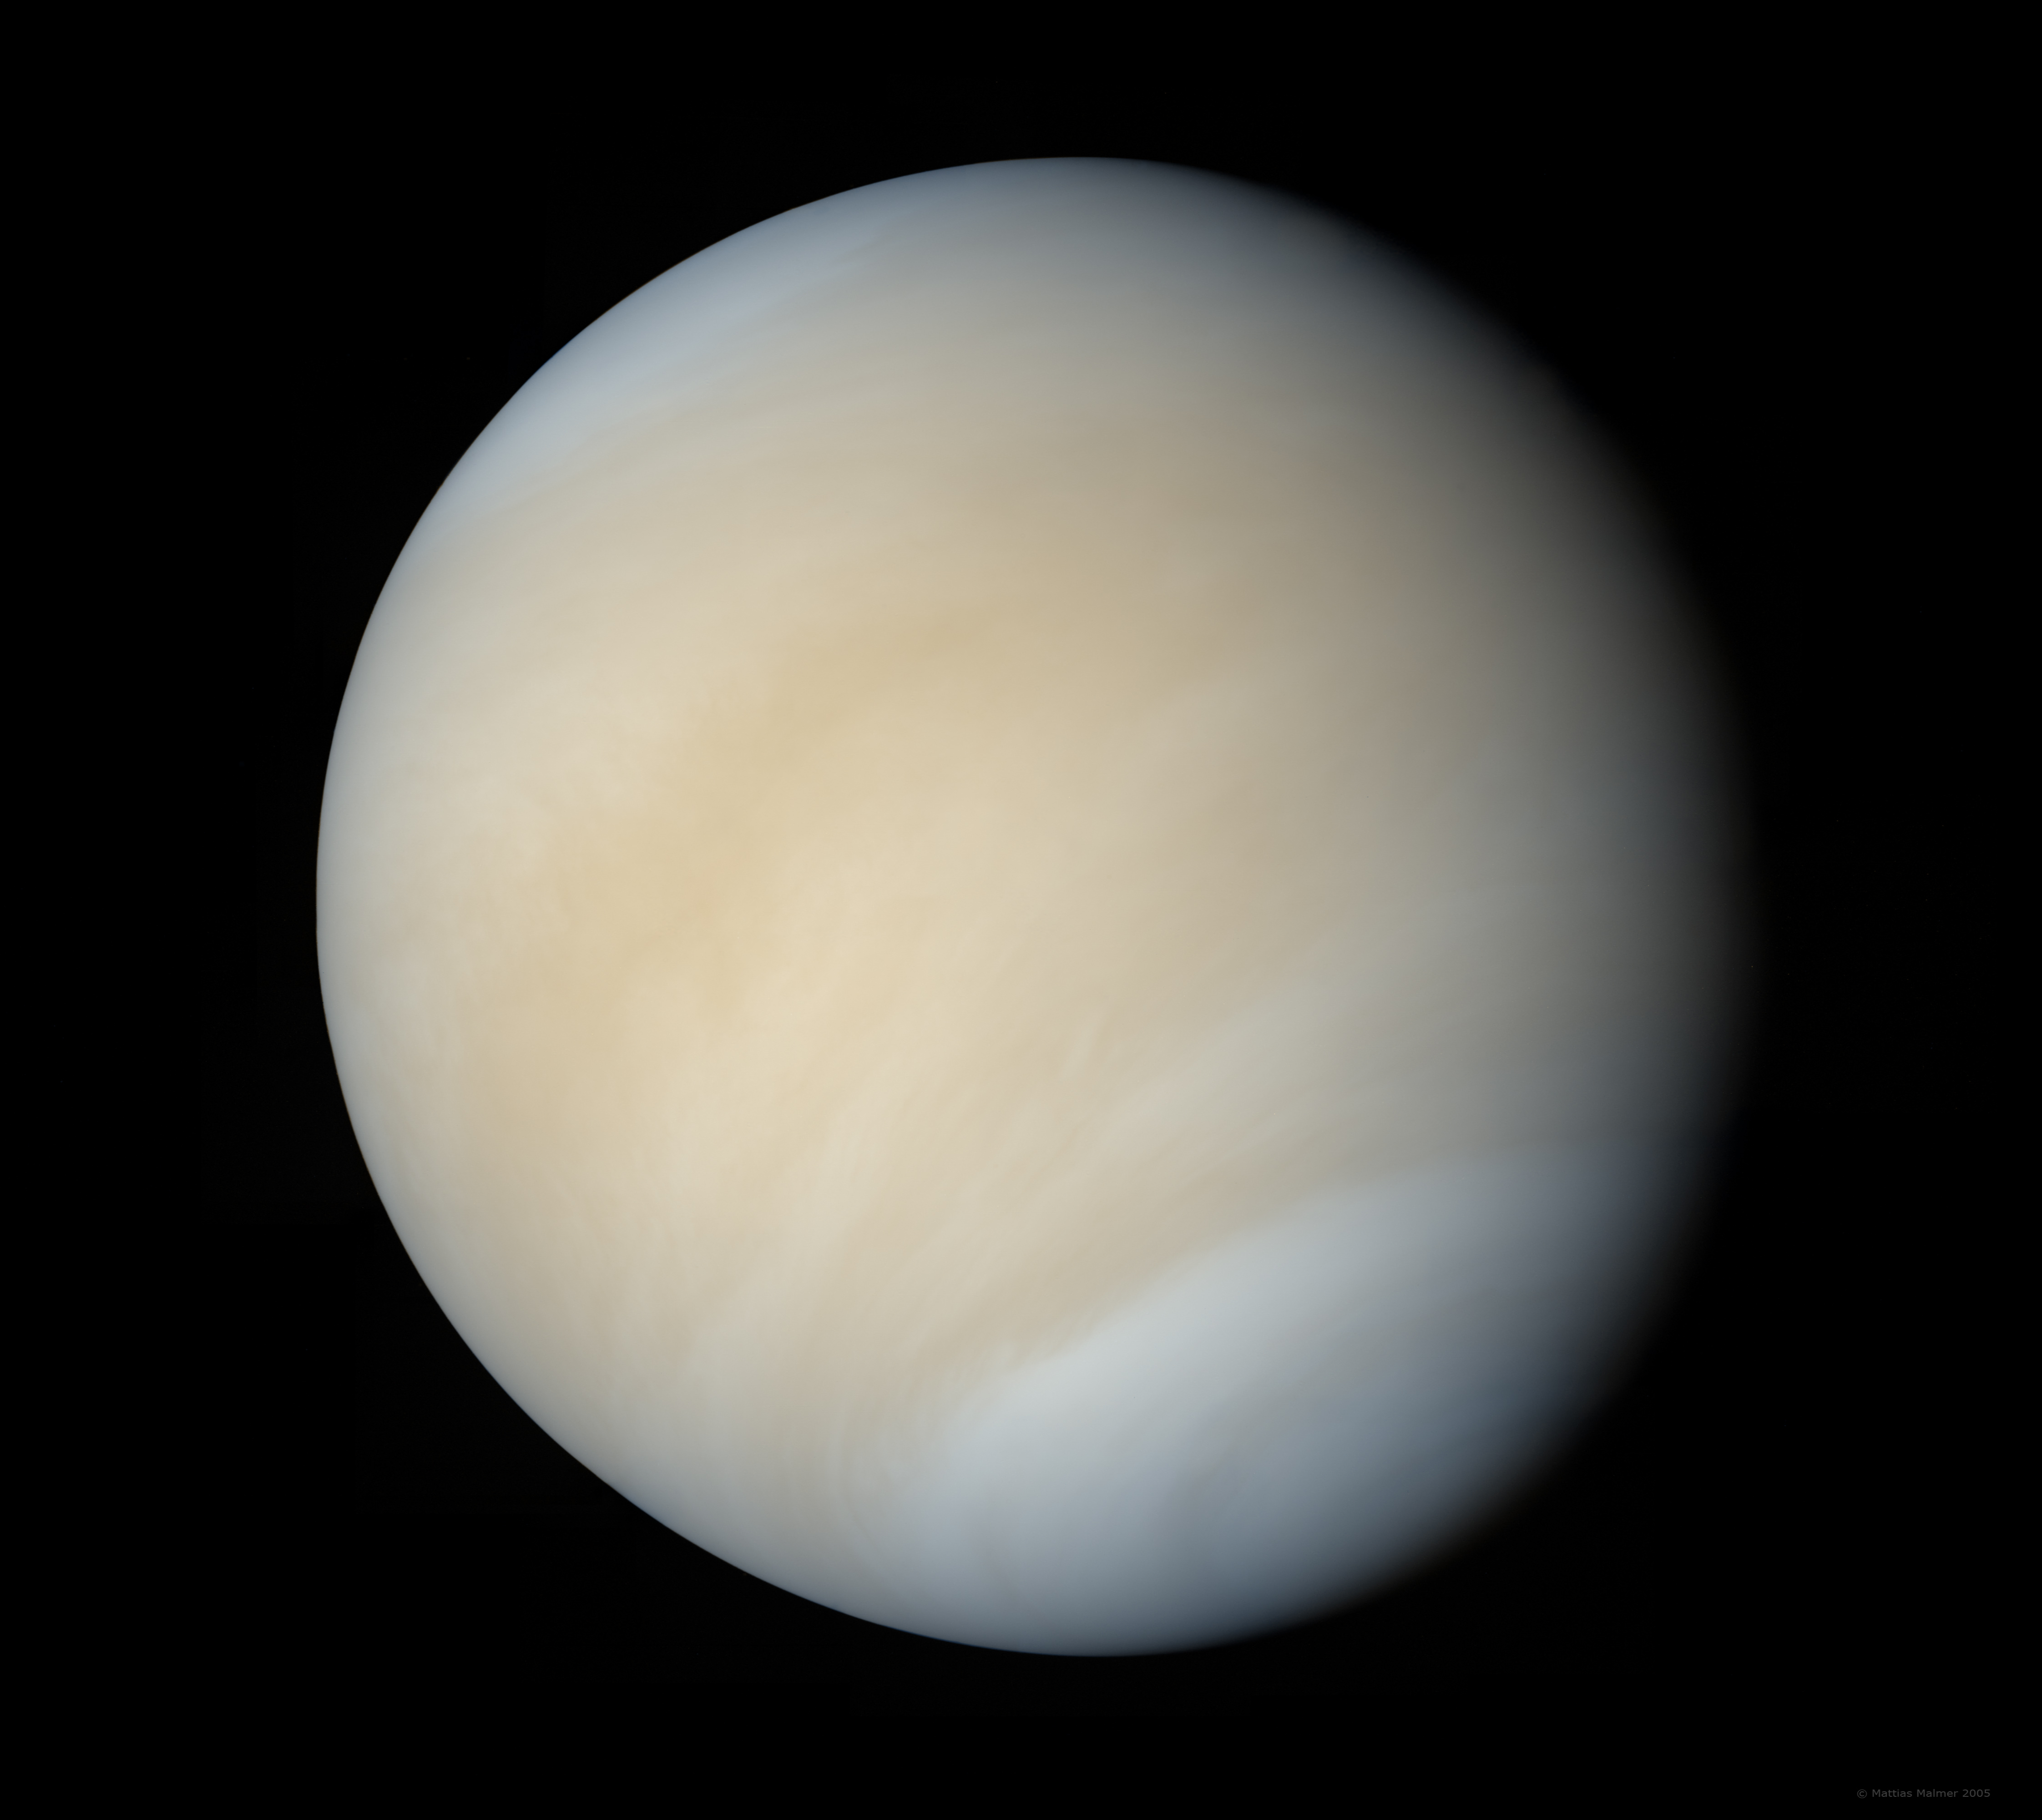
\includegraphics[width=0.4\textwidth]{venus.jpg}\hspace{0.05\textwidth}
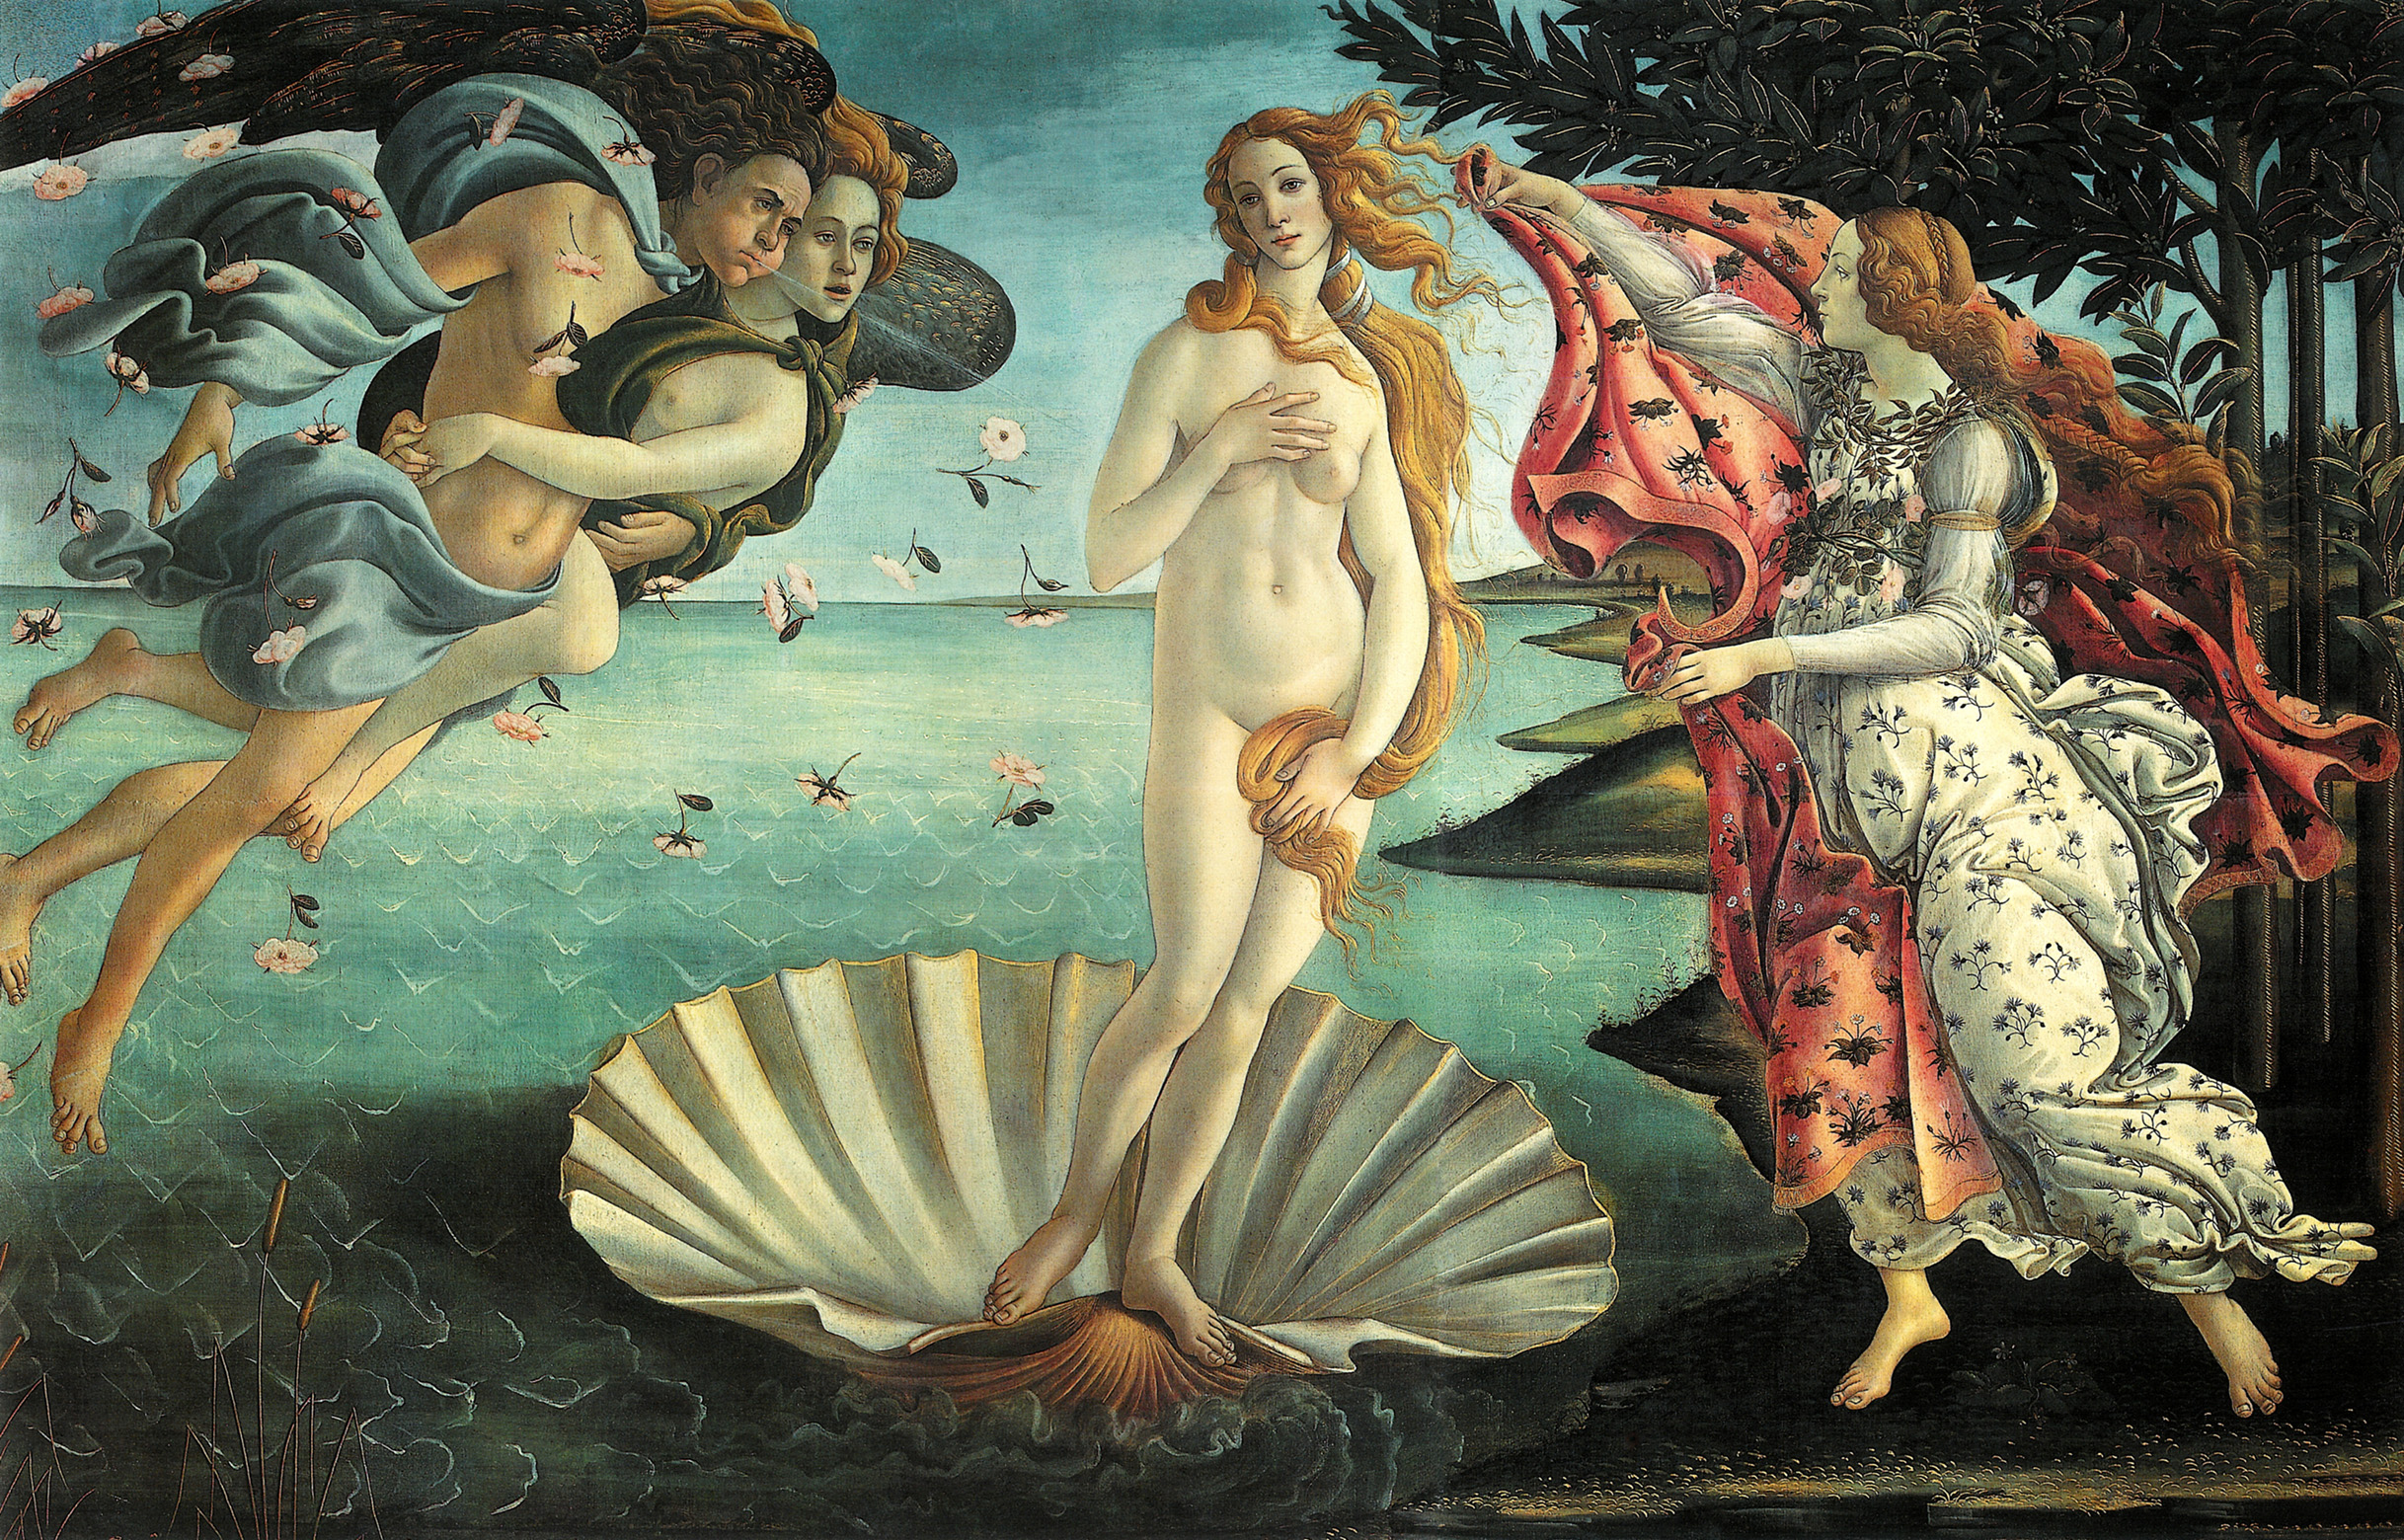
\includegraphics[width=0.5\textwidth]{birth-of-venus.jpg} \\

\url{https://www.youtube.com/watch?v=PyBkzZoMYN4}
\EC
}

\frame{\frametitle{\bf Beautiful, lovely Venus...}

\large
\BI
\pause
\item The surface temperature is hot enough to melt lead
\pause
\item It rains sulfuric acid
\pause
\item The atmospheric pressure is high enough to crush bone
\pause
\item ... if there is a Hell in our solar system, it is Venus. What in Hell -- literally -- happened?
\EI
}

\frame{\frametitle{\bf Horrifying, poisonous Venus...}

\begin{columns}
\column{0.5\textwidth}
\BI
\item Visible light doesn't go through this atmosphere well
\item ... radar does!
\item We've used radar to map the Venusian surface
\item It has some interesting geology
\item You can read about it in your book
\EI
\column{0.5\textwidth}
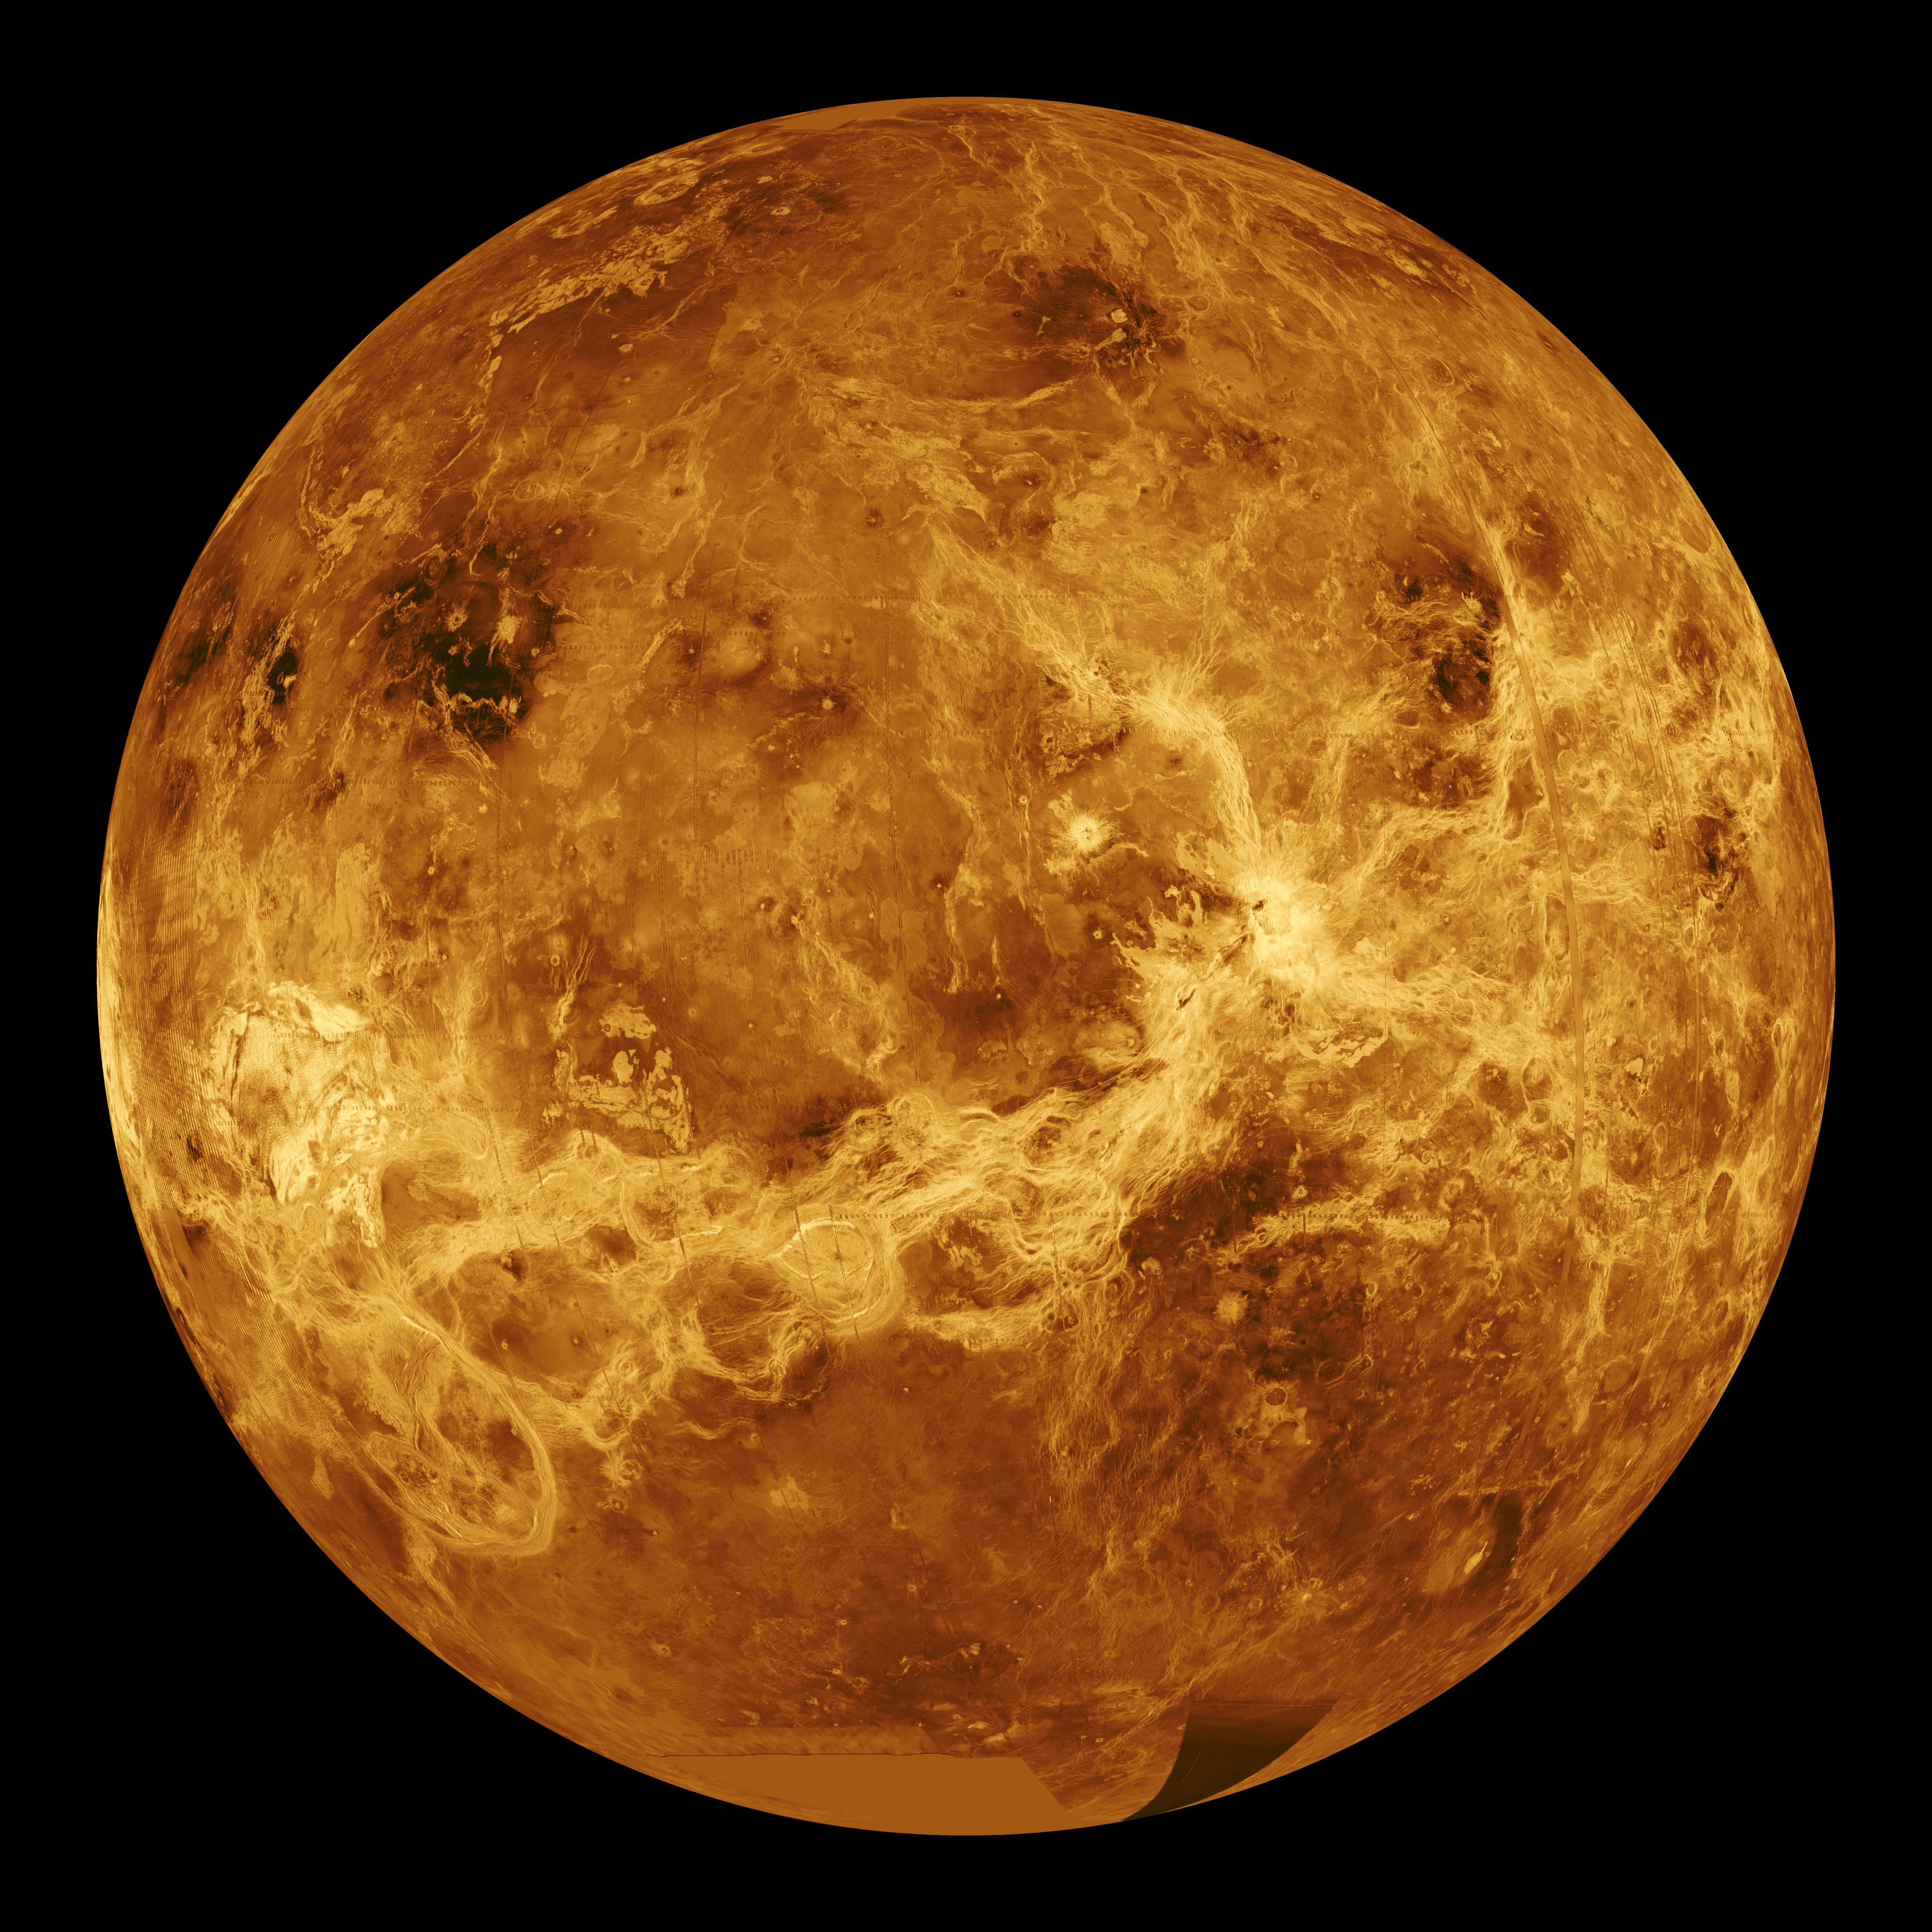
\includegraphics[width=0.99\textwidth]{venus-radar.jpg}
\end{columns}
}

\frame{

\BC
\large
Earth, cradle of life...

\BS

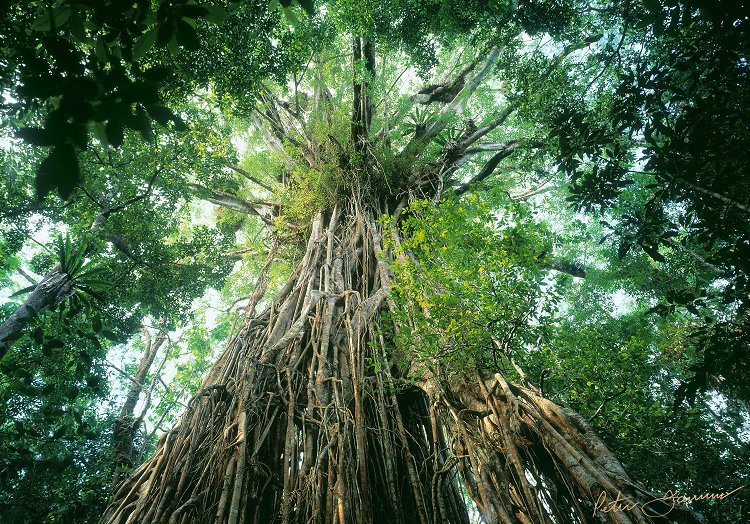
\includegraphics[width=0.55\textwidth]{cathedral-fig.jpg}\hspace{0.04\textwidth}
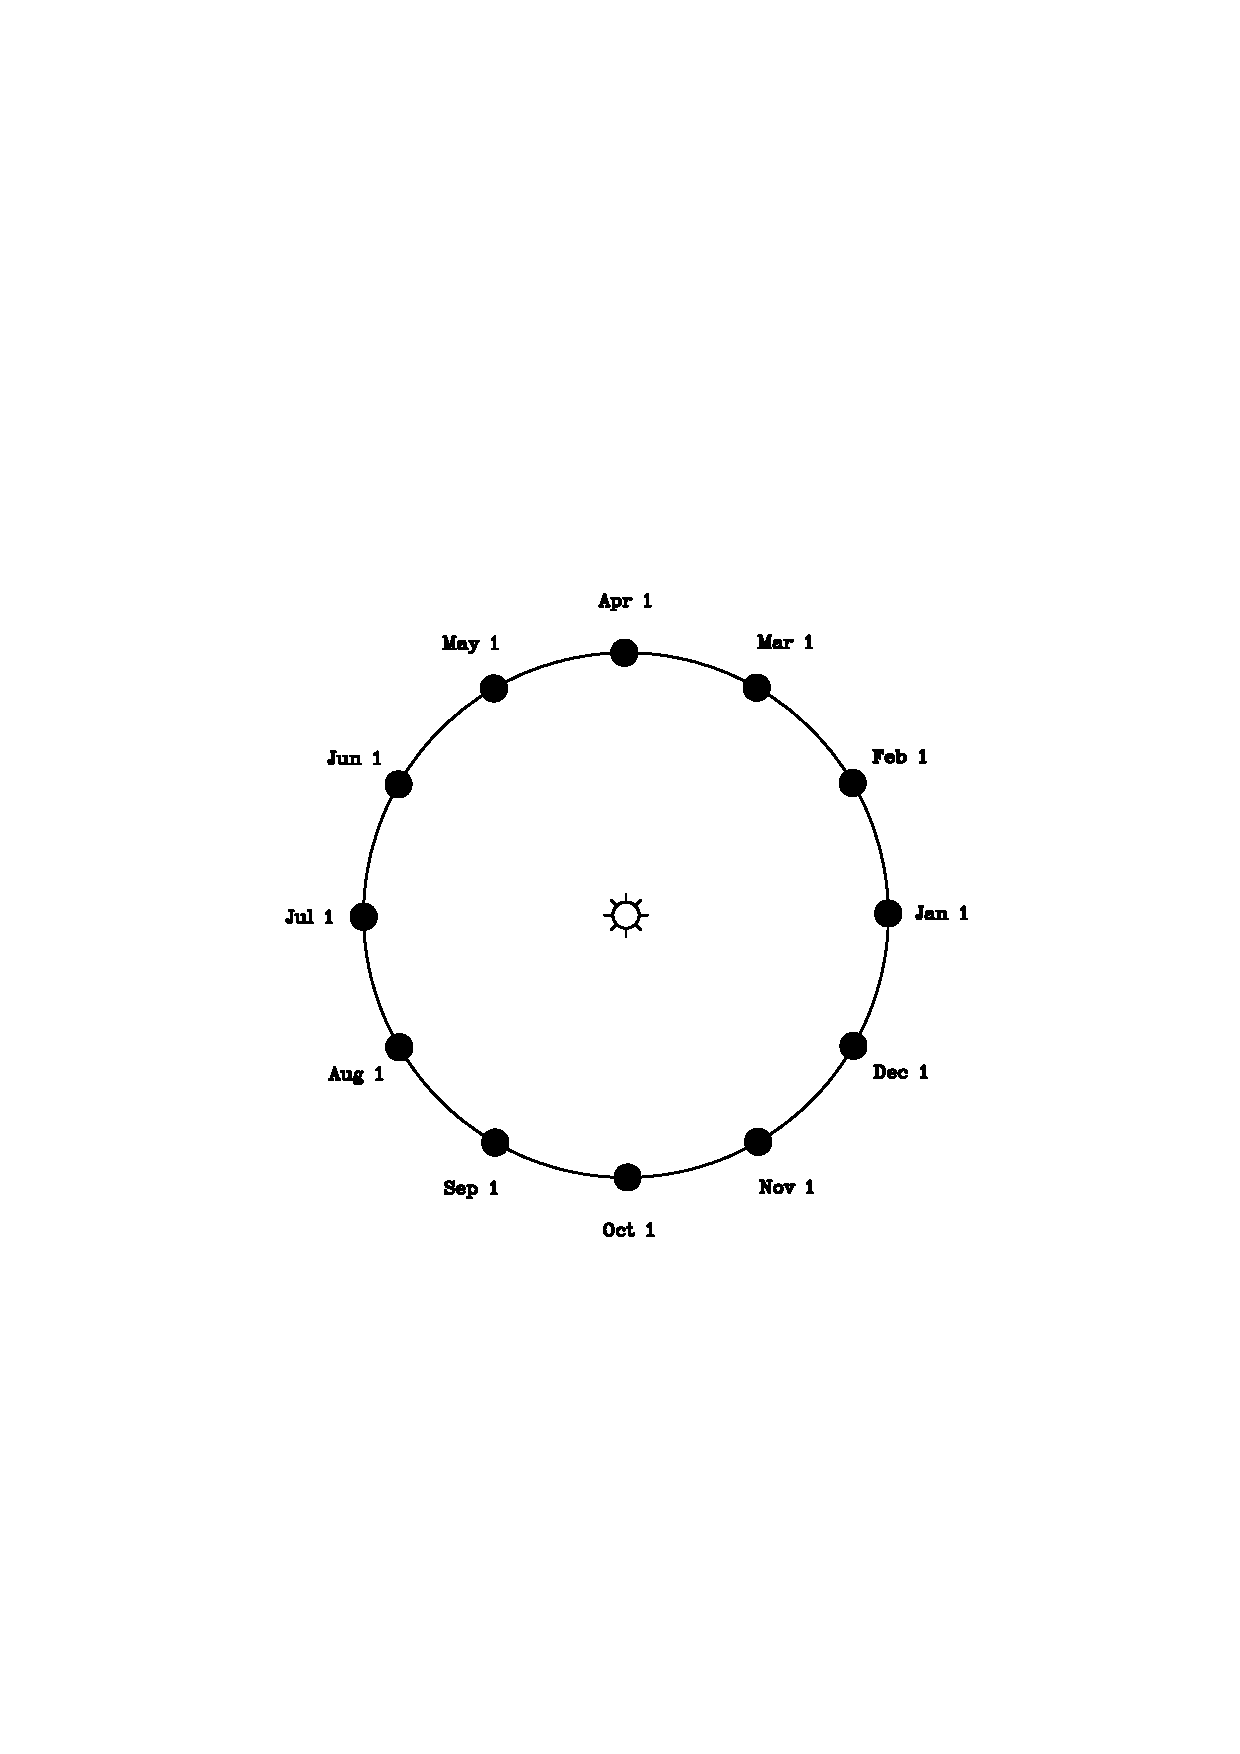
\includegraphics[width=0.4\textwidth]{earth.jpg} \\

\BS

\url{https://www.youtube.com/watch?v=MbHQ6eWANIo} (not by Holst!)

\EC

}

\frame{\frametitle{\bf Earth, our home...}

\BI
\item Active volcanism throughout its history
\item Large amounts of liquid water on surface
\item Stable climate: most of surface between 273 K and 373 K (freezing/boiling) for a long time
\item Atmosphere with significant oxygen, nitrogen, some $\rm CO_2$
\pause
\item Surface covered by self-replicating, reactive, diverse, beautiful, {\it aware} machines, made of carbon compounds: {\it life!}
\item Atmospheric oxygen from the byproducts of plant metabolism
\item Hot core generates a magnetic field that shields atmosphere from solar wind
\EI
}

\frame{\frametitle{\bf Our large Moon...}

\BI
\item The Moon appears to have similar composition to Earth
\item ... but it lacks active geology or an atmosphere
\pause
\item Shortly after the formation of Earth, something the size of Mars hit us
\item Some of the resulting fragments broke off and orbited the Earth
\item They coalesced into the Moon
\EI

\BS

\BC
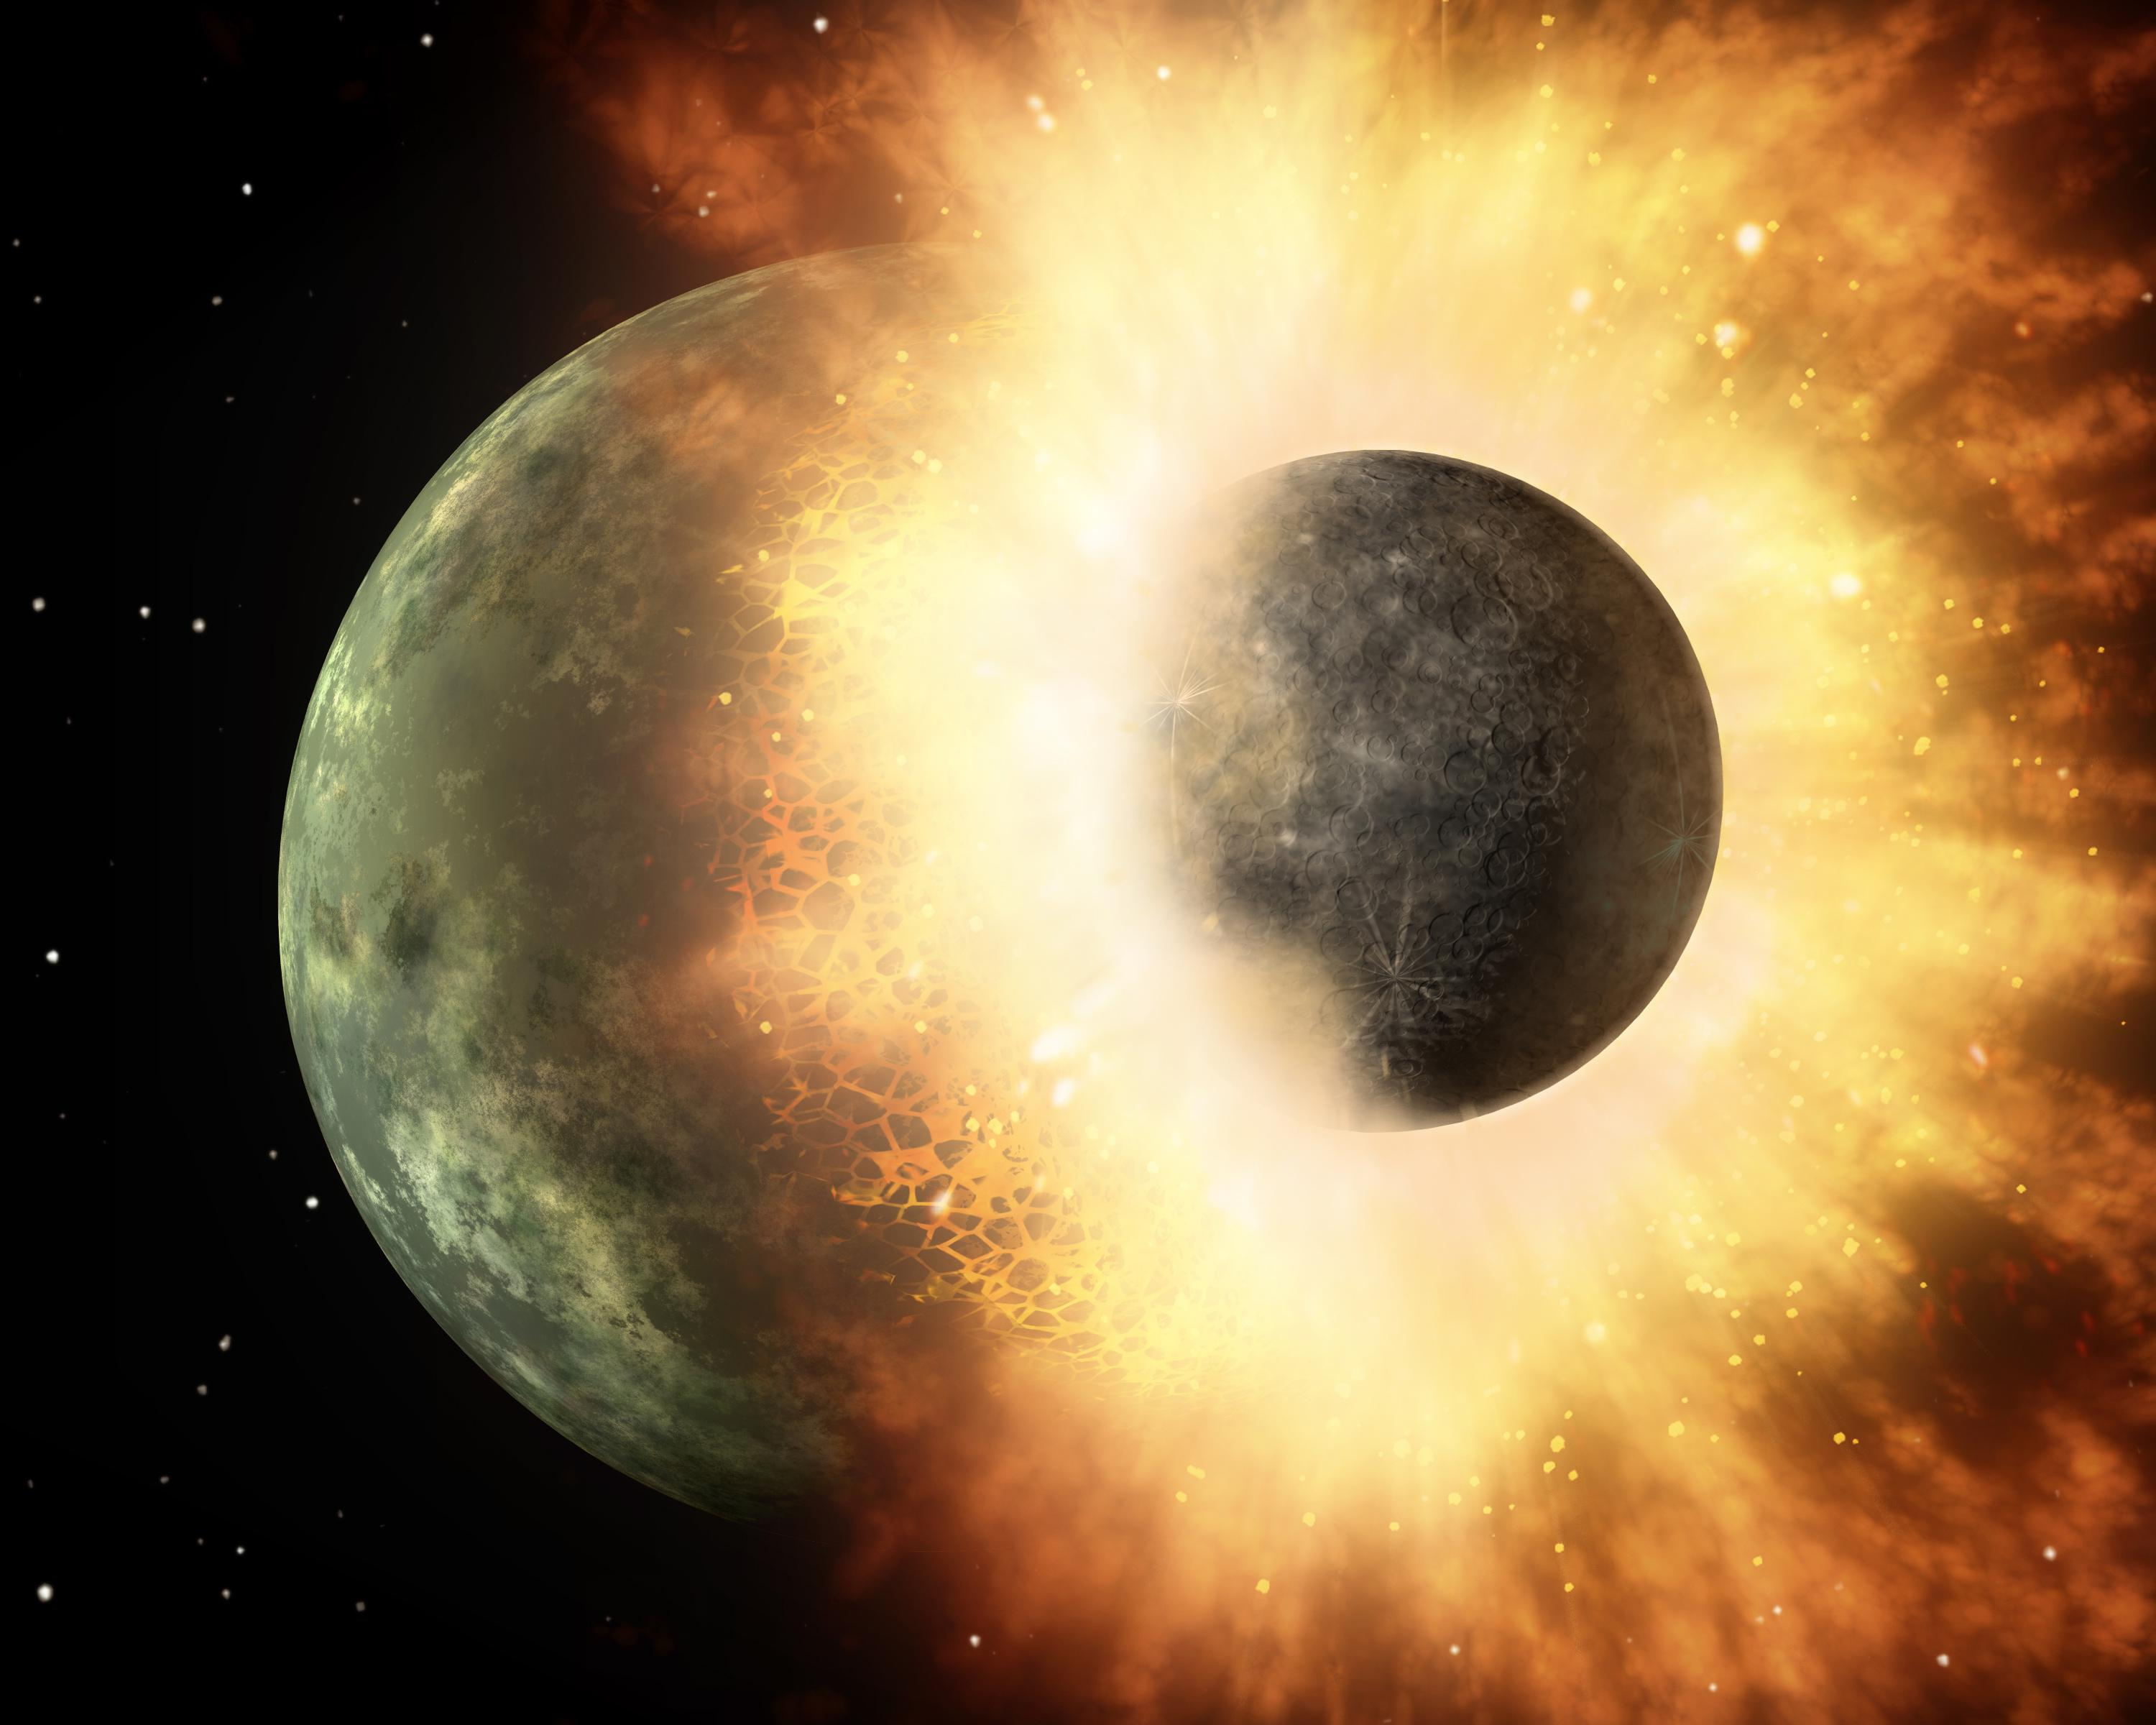
\includegraphics[width=0.6\textwidth]{impact.jpg}
\EC
}

\frame{\frametitle{\bf The greenhouse effect}

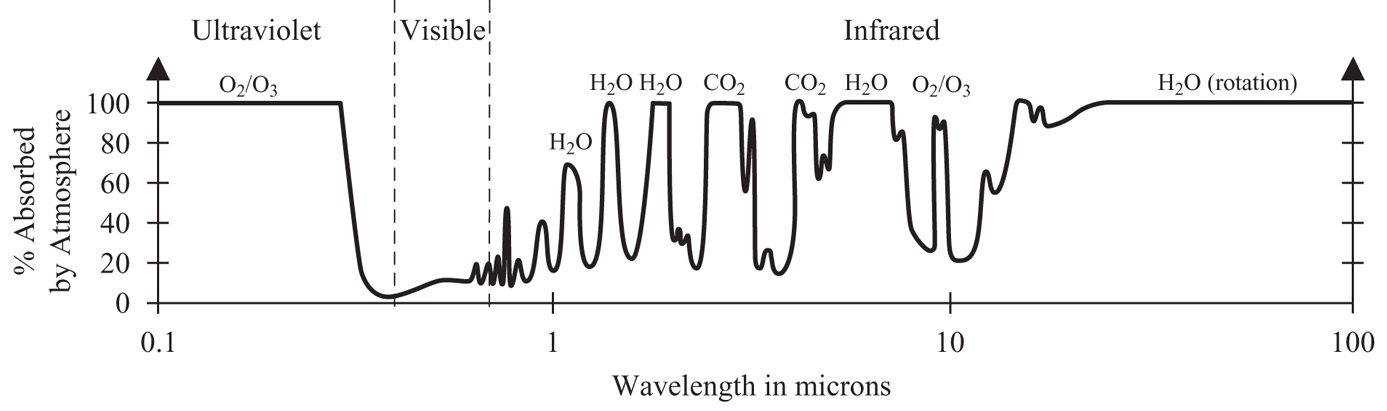
\includegraphics[width=\textwidth]{absorption.jpg}

\BI
\item As you saw/will see in lab this week: planets' temperature set by radiation balance:
\BI
\item Incoming thermal radiation from Sun -- visible
\item Outgoing thermal radiation from planet -- infrared
\EI
\item What happens if you have an atmosphere that reflects IR, but not visible light?
\item The outgoing thermal radiation is greatly reduced!
\EI

\BS

\BC
\large
This is called the {\it greenhouse effect}.
\EC
}

\frame{\frametitle{\bf The greenhouse effect}
Venus has a {\it tremendously thick} atmosphere and a powerful greenhouse effect.

\BI
\item Its atmosphere contains a great deal of $\rm CO_2$, which reflects IR strongly
\item The thermal radiation that would carry heat away from Venus can't get out
\item It is over 400 K hotter than was predicted by the calculation you are doing this week
\EI

\BS

Earth has a {\it thinner} atmosphere.

\BI
\item Nitrogen doesn't absorb strongly at any relevant wavelengths
\item $\rm H_2 O$ and $\rm CO_2$ are strong greenhouse gases, but they are only a bit of the atmosphere
\item We are about 20 K warmer than predicted by that crude math
\item These gases are very important for determining Earth's temperature!
\EI
}

\frame{\frametitle{\bf The greenhouse effect}

\BC
\Huge
Complete {\it Lecture Tutorials} pp. 105-110.
\EC
}



\end{document}
